OpenGL insights chapter 22



\chapter{Voxel-based Global Illumination}
Light propagation volumes (see chapter \ref{chp:lpv}), precomputed radiance transfer (see chapter \ref{chp:prt}), etc., these kinds of methods based on that low-frequency lighting can be represented as low order SH basis, such as environment maps and large area light, etc.. This assumption is also the limitation of these methods.

Global illumination is computationally expensive for several reasons. It requires computing visibility between arbitrary points in the 3D scene, which is difficult with rasterization based rendering. Secondly, it requires integrating lighting information over a large number of directions for shaded point.

Voxel cone tracing, which has been proposed by Cyril Crassin\cite{a:InteractiveIndirectIlluminationUsingVoxelConeTracing}, et al. in 2011, uses a hierarchical voxel octree to approximate the real scene meshes to reach a fast estimation of the visibility and incoming energy. And it uses MIP mapping technique to pre-filter the incoming lighting to speed up the integrating over a large directions. 

Besides, this method update the octree on the fly, so it can computing indirect lighting in real-time that avoids costly precomputation steps. And it is also not restricted to low-frequency illumination. By using a regular octree to approximate the scene and an interactice octree-voxelization scheme, it exhibits an almost scene-independent performance and can handle complex scenes with dynamic content.

What a smart and an elegant method on global illumination! Since it came out, it first had been integrated into Unreal Engine 4\cite{a:TheTechnologyBehindtheUnrealEngine4Elementaldemo} (right now they have removed this method because of the performance, they have been using a new technique names distance field global illumination which will be introduced in the next chapter), and now it's been implementing in CryEngine 3\sidenote[][-2mm]{\url{http://docs.cryengine.com/display/SDKDOC2/Voxel-Based+Global+Illumination}}, which has removed it's previous global illumination technique, light propagation volumes. Another case is the up coming game "The tomorrow children"\cite{a:TheTechnologyofTheTomorrowChildren}, which implements a modification of the original voxel cone tracing technique.




\section{Ray Tracing with Cones}
Before we go into voxel cone tracing algorithm, we should first know the core idea of it: \textit{cone tracing}. In fact, it has been proposed since 1984 by John Amanatides\cite{a:RayTracingwithCones}. And it is still an important technique which has been widely used, such as in voxel-based global illumination which is being described in this chapter, and in distance field global illumination in Unreal Engine 4 which will be introduced in the next chapters.


\subsection{The Problem of Ray Tracing}
In ray tracing, rays are shot from the eye into the world, see figure \ref{f:ray-tracing-vs-cone-tracing}(a). They are constrained so that they pass through the center of the pixels in the virtual screen. Once they have left, any relationship between the ray and the pixel on which the result will be displayed is severed. This is because a ray is defined as a starting point and a direction which together from a line. This simple definition allows for straightforward and fast intersection calculations with various objects. Unfortunately, it also has drawbacks.

\begin{figure}\label{f:ray-tracing-vs-cone-tracing}
	\begin{subfigure}[b]{0.47\textwidth}
		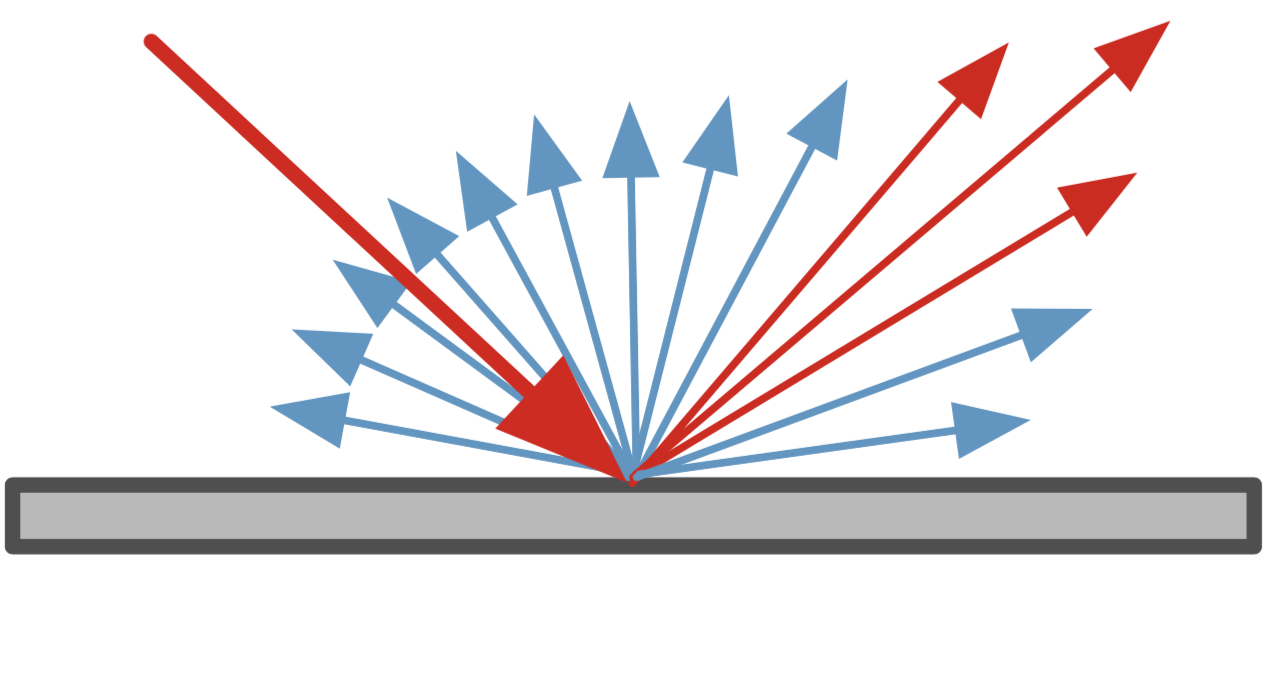
\includegraphics{graphics/vct/vct-1-1}
		\caption{Ray tracing: many rays}
	\end{subfigure}
	\begin{subfigure}[b]{0.53\textwidth}
		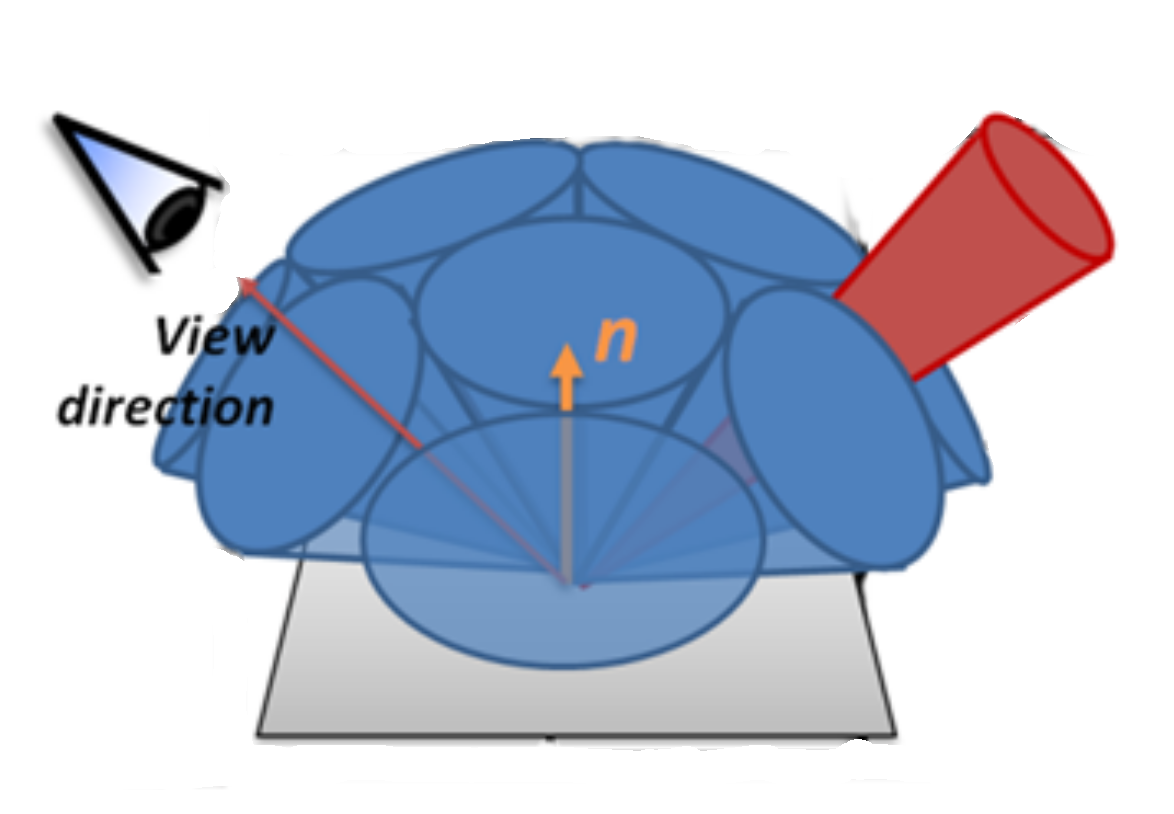
\includegraphics{graphics/vct/vct-1-2}
		\caption{Cone tracing: few large cones}
	\end{subfigure}
	\caption{Ray tracing compared to cone tracing. In ray tracing, when the ray reaches the intersection point, it stops. While in cone tracing, it accumulates the values of the intersection area alone the cone direction. Large groups of rays can be approximated by a single cone, so less traces are required.}
\end{figure}

The main drawback with the above standard approach is that there is not enough information associated with the ray to perform anti-aliasing. Rays allow us only to sample at the one point in the center of a pixel. There is no way of knowing or calculating what else is visible in neighborhood surrounding the sample point.

The only way to anti-alias within standard ray tracing is to go to higher resolution. Whitted proposed adaptive supersampling\cite[-4mm]{a:ray-tracing}. However, there are a couple of problems associated with this approach. First, the amount of computation can go up drastically in pixels where large variances of intensity occur. The second problem is that small details may "fall through the cracks" of the sample points. This is especially true of objects that are reflected or refracted by other objects.

One way of attacking the sampling problem outlined above is to modify the definition of "ray" to a cone, see figure \ref{f:ray-tracing-vs-cone-tracing}(b). The pixel should represent not a point but an area of the screen. Intersection calculations between this extended ray and an object can decide not only if there is an intersection but also what fraction of the ray intersects the object. This fractional coverage information is sufficient to perform simple area anti-aliasing. Also, nothing can "fall through the cracks" as the ray covers the whole pixel.  



\subsection{How Does It Work?}
So, how does exactly it works? For both techniques, we're trying to obtain a number of samples of the incident radiance at a point by shooting out primitives, and intersecting them with the scene, see figure \ref{f:rays-and-cones}.

\begin{figure}\label{f:rays-and-cones}
	\begin{center}
		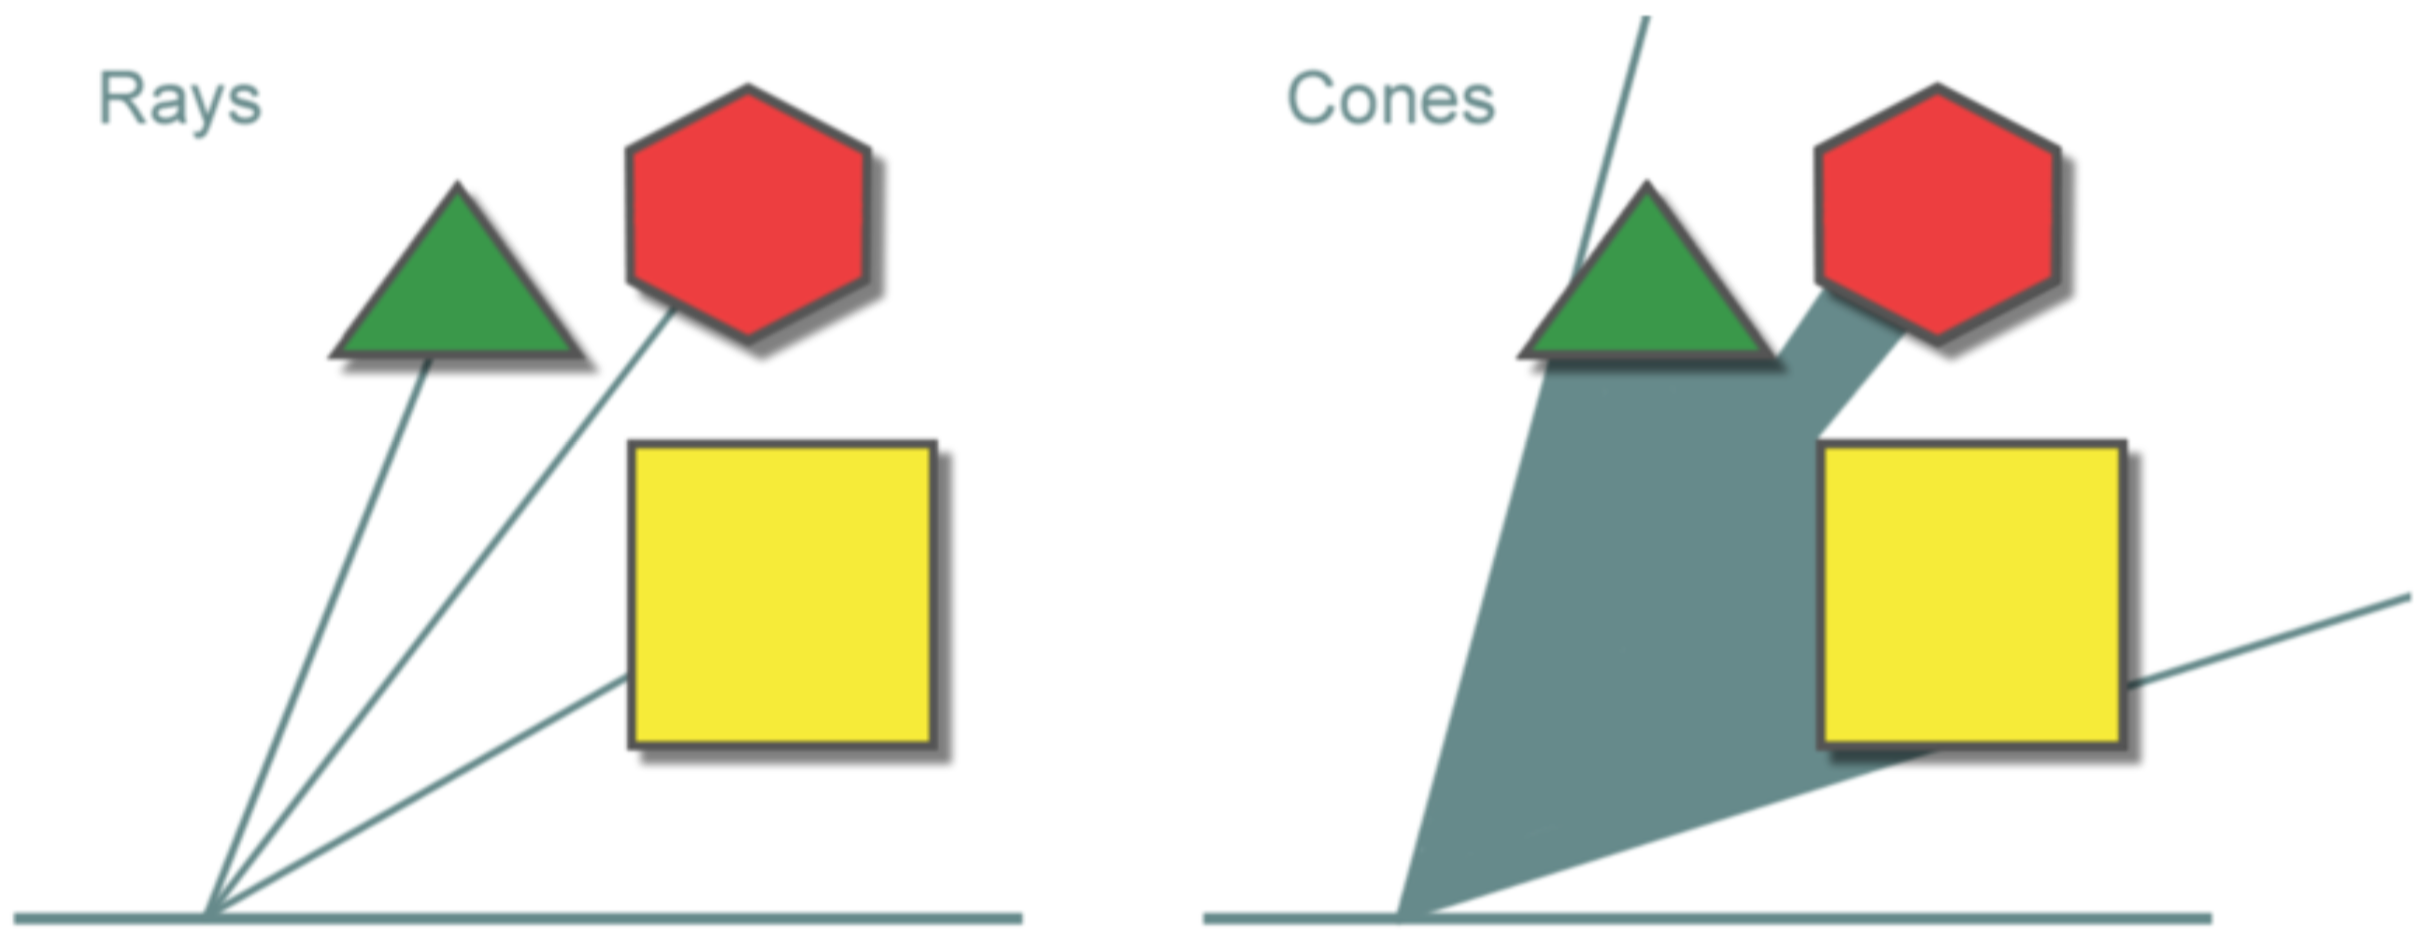
\includegraphics[width=0.8\textwidth]{graphics/vct/vct-2-1}
	\end{center}
	\caption{With a ray the intersection is at a point, where as with a cone, it ends up being an area or perhaps a volume, depending on how you are thinking about it.}
\end{figure}

If we take enough well distributed samples, then we can combine them together to form an estimated for the incident lighting at our point, which we could then feed through a BRDF that represented the material properties at out point, and calculate the exitant lighting.

So the key difference between the two approaches is what happens when we evaluate the intersection of our primitives with the scene. With a ray the intersection is at a point, where as with a cone, it ends up being an area or perhaps a volume (depending on how you are thinking about it).

The important thing, is that because it's no longer a point, the properties of our estimate change. Firstly, we aren't necessarily looking in just one location in the scene for our intersection anymore, we can have multiple partial hits by our cone.

And secondly, because of the need to evaluate the scene over an area, our scene has to be filterable. Also, because we are filtering we are no longer getting an exact value, we are getting an average, and so the accuracy of our estimate goes down.

But on the upside, because we are evaluating an average, the noise, that we would typically get from ray tracing, is largely absent.



\subsection{How Do We Sample?}
So obviously the challenge is, how do we sample from our cone. The purple surface area in the picture \ref{f:cone-sample} defining where we intersect is not a very easy thing to evaluate. 

\begin{figure}\label{f:cone-sample}
	\begin{center}
		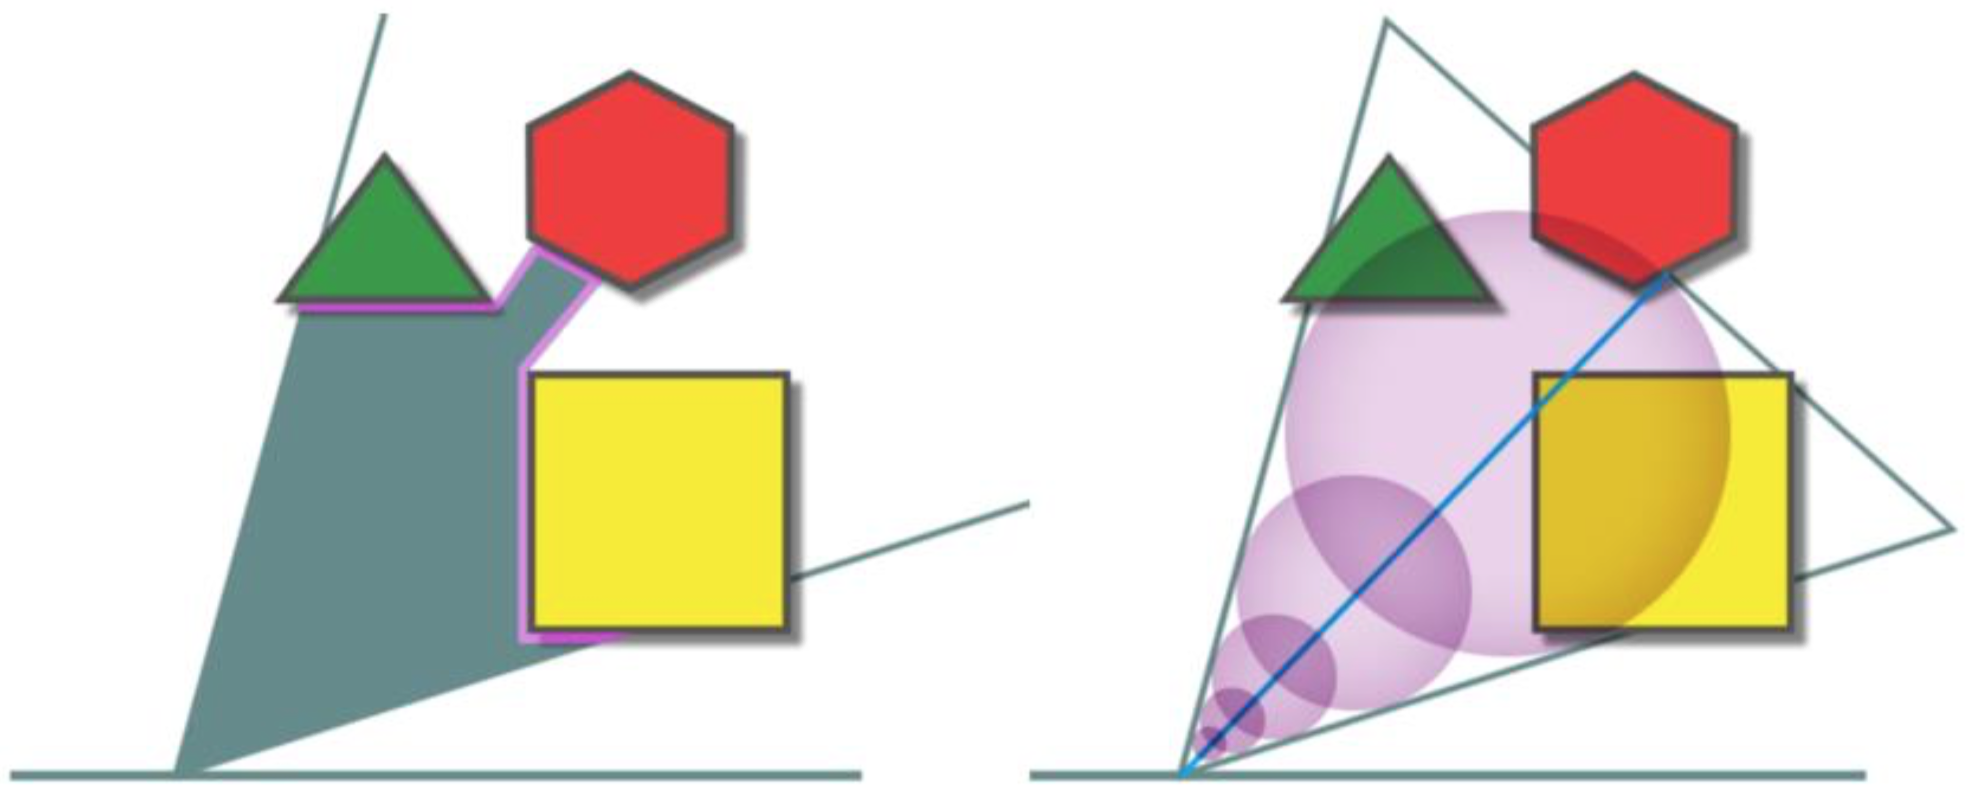
\includegraphics[width=0.8\textwidth]{graphics/vct/vct-2-2}
	\end{center}
	\caption{Cone tracing accumulate each volume samples as it marches along the cone.}
\end{figure}

So instead, we take a number of \textit{volume samples} along the cone, with each sample returning an estimate of light reflected towards to apex of the cone, as well as an estimate of the occlusion in that direction. It turns out that we can combine these samples with the same basic rules we would use for ray marching through a volume.




\subsection{Accuracy Issues}
One thing worth noting is that because we are using volume samples, we are potentially going to get inaccurate results in the case where we have a cone that is partially occluded, as we don't carry any information about the shape of the occlusion onto the next sampling step.

\begin{marginfigure}
	\begin{center}
		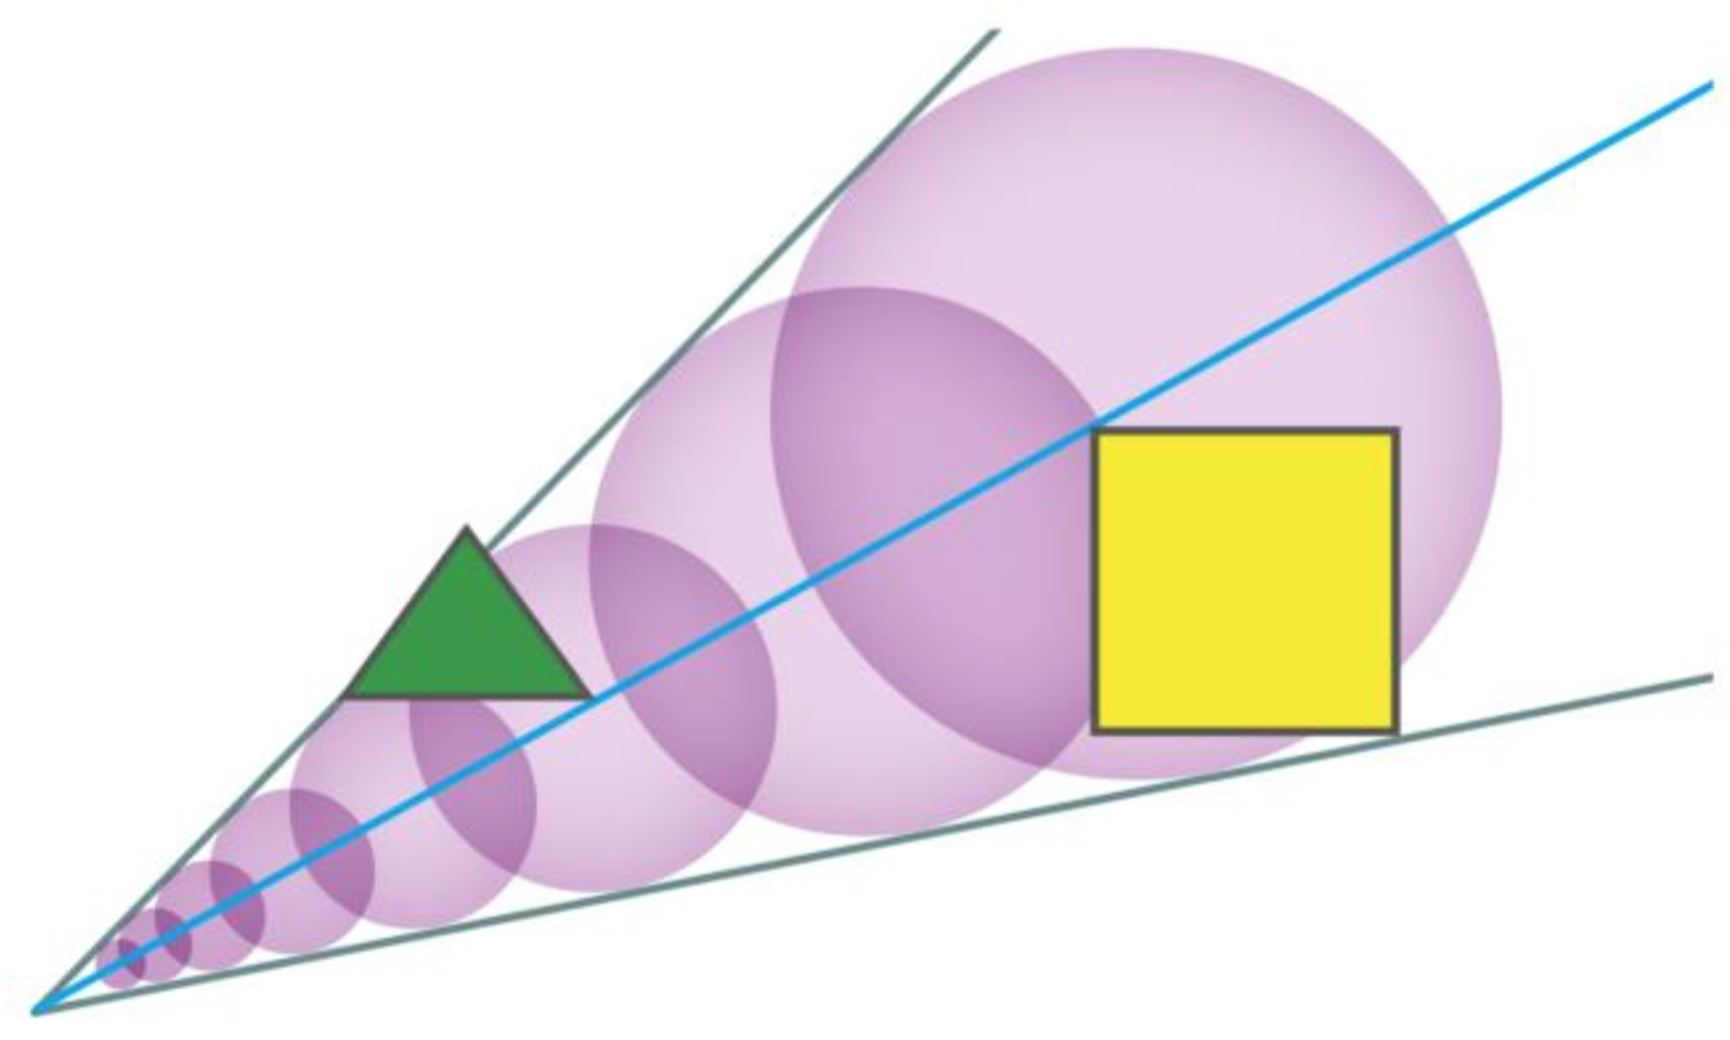
\includegraphics[width=1.0\textwidth]{graphics/vct/vct-2-3}
	\end{center}
	\caption{$0.5*0.5=0.25$, incorrect!}
	\label{f:cone-issues}
\end{marginfigure}

So in this example, see figure \ref{f:cone-issues}, we have two partial occlusions of our cone, both of them occlude 50\% of the light from the sky. But as you can see in reality, if we were combine these two, we should get 100\% occlusion of light. Where as our cone trace will actually tell us that we can still see 25\% of the light, because all we do is just naively combine their occlusion in the same way we would with alpha blending.

This doesn't tend to be such a big issue in practice, but it is worth bearing in mind that cone tracing is only a very rough estimate. 






\section{Volumetric Geometry Representation}
Obviously, by using cone tracing, we can speed up the visibility computation and integrating over a large directions. But we also need an acceleration structures of scene representation, instead of the real scene meshes, which can work with cone tracing friendly. 

\begin{marginfigure}
	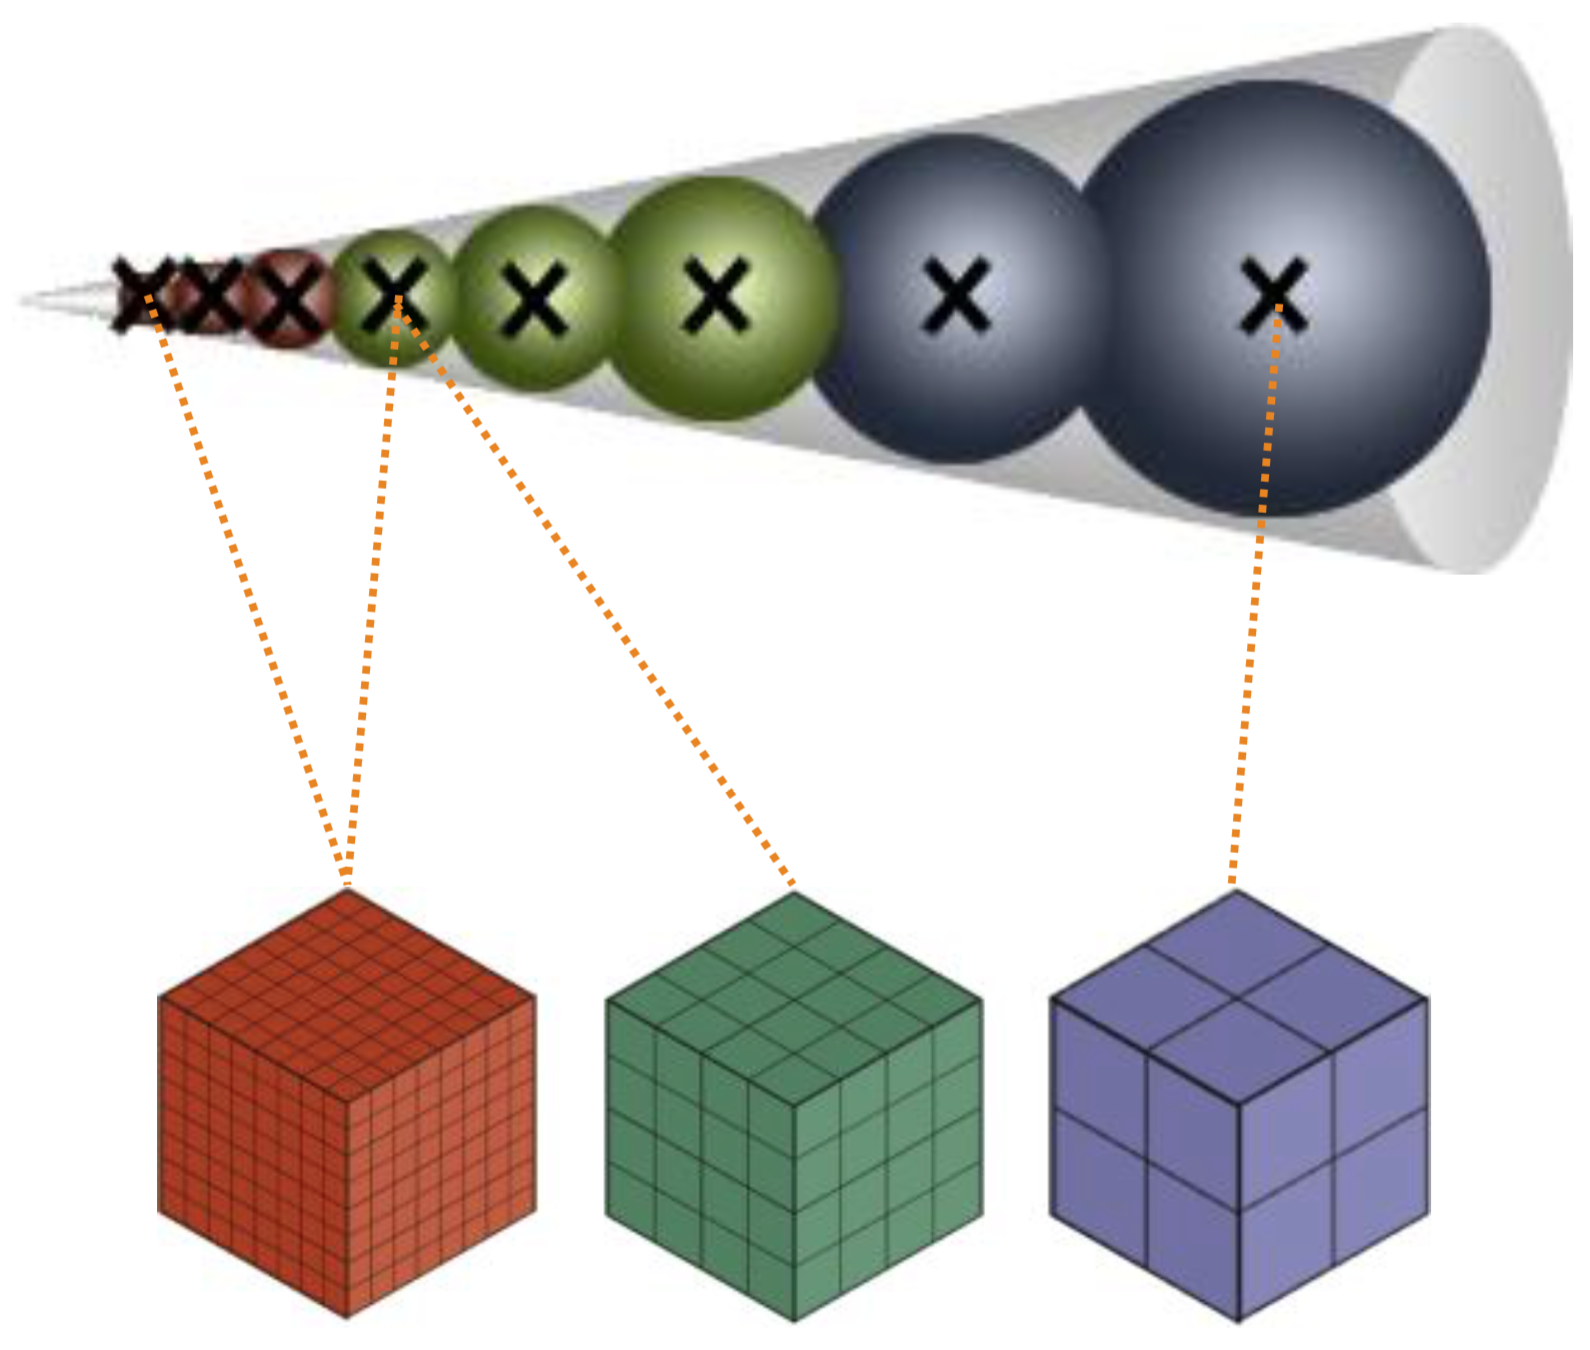
\includegraphics{graphics/vct/vct-2-4}
	\caption{In every step of cone tracing march, it uses the pre-filtered irradiance directly from a pre-filtered scene representation.}
	\label{f:vct-pre-filtered-data}
\end{marginfigure}

But what exactly do we need? Now we know what we need to do is accumulating our irradiance data as we march along our cone. Accumulating an area means that we need pre-filter this areas in each march step. So all we need is a pre-filtered representation of the whole scene, that in every step of march, we can get this pre-filtered results, the average of this area, directly, see figure \ref{f:vct-pre-filtered-data}.


That's the whole idea of voxel-based global illumination. In this algorithm, they use a voxel octree to represent the scene and pre-filter the radiance into this structure. Then cone trace the octree to get occlusion and indirect lighting informations. 

In this section, we'll detail the hierarchical voxel structure. How is it chose, how to pre-filter the needed datas, and how is the voxel represented, etc..




\subsection{Voxel-based Approach to Geometry Pre-filtering}
As we have described in the previous section, we need to pre-filter the mesh representation of the scene so we can use cone tracing to speed up the light transfer computation. 

\begin{marginfigure}
	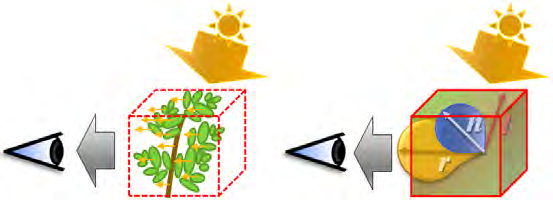
\includegraphics{graphics/vct/vct-4-1}
	\caption{Illustration of the pre-filtering of complex geometrical details inside a single voxel element in order to allow the reconstruction of an overall shading contribution.}
	\label{f:vct-pre-filtering-assumption}
\end{marginfigure}

The idea of pre-filtering is that, under some linearity assumptions, it is possible to factor some shading parameters out of the shading computation when integrating it over an area (in this case a pixel), and to pre-integrate (average) these parameters separately. This permits us to remove detail frequencies higher than the rendering resolution while preserving the mean value of the pixel footprint. Such geometry pre-filtering would provide a scalable rendering solution with an amount of rendered data depending only on the rendering resolution, and thus scaling up to very complex scenes.

The key observation that allow the pre-filtering of geometry was made by Perlin\cite{a:hypetrtexture} and by Kajiya and Kay\cite[5mm]{a:Renderingfurwiththreedimensionaltextures}. When considering a given volume of space containing multiple surfaces more or less randomly distributed (like the branch and leaves illustrated in figure \ref{f:vct-pre-filtering-assumption}), exact positions of surfaces inside this volume do not really matter when computing the overral light interaction within this volume. Thus, only using an overall density distribution and overall reflectance function is enough to accurately compute the interaction of light with this volume (see figure \ref{f:vct-pre-filtering-assumption}).

Then, when sets of complex surface definitions are considered, the parameters used for computing illumination for such sets can more easily be described volumetrically, for a given volume containing these surfaces, than with a simplified surface definition. With such volumetric representation, the matter is represented by a density distribution associated with the parameters for the shading model describing the way light is reflected within a unit of volume, instead of a set of interfaces and parameters on them. Once the geometry is transformed into density distribution, filtering this distribution becomes a simple linear operation. 

\begin{marginfigure}
	\begin{center}
		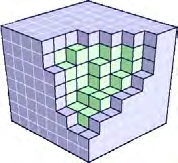
\includegraphics[width=0.7\textwidth]{graphics/vct/vct-4-2}
	\end{center}
\end{marginfigure}

The name \textit{voxel} comes from "volumetric elements" and it represents the generalization in 3D of the pixels. Voxels represent the traditional way to store volumetric data. They are organized in axis-aligned grids subdividing and structuring space regularly. Voxel representations offer a promising way to store volumetric data in order to unify texture and geometrical representations, while simplifying filtering. The significant advantage of voxels is the richness of this representation and the very regular structure which makes it easy to manipulate. That makes voxels a good candidate to address aliasing issues that are hard to deal with in triangulated models.

\begin{figure}\label{f:vct-voxel-based-pre-filtering}
	\begin{subfigure}[b]{1.\textwidth}
		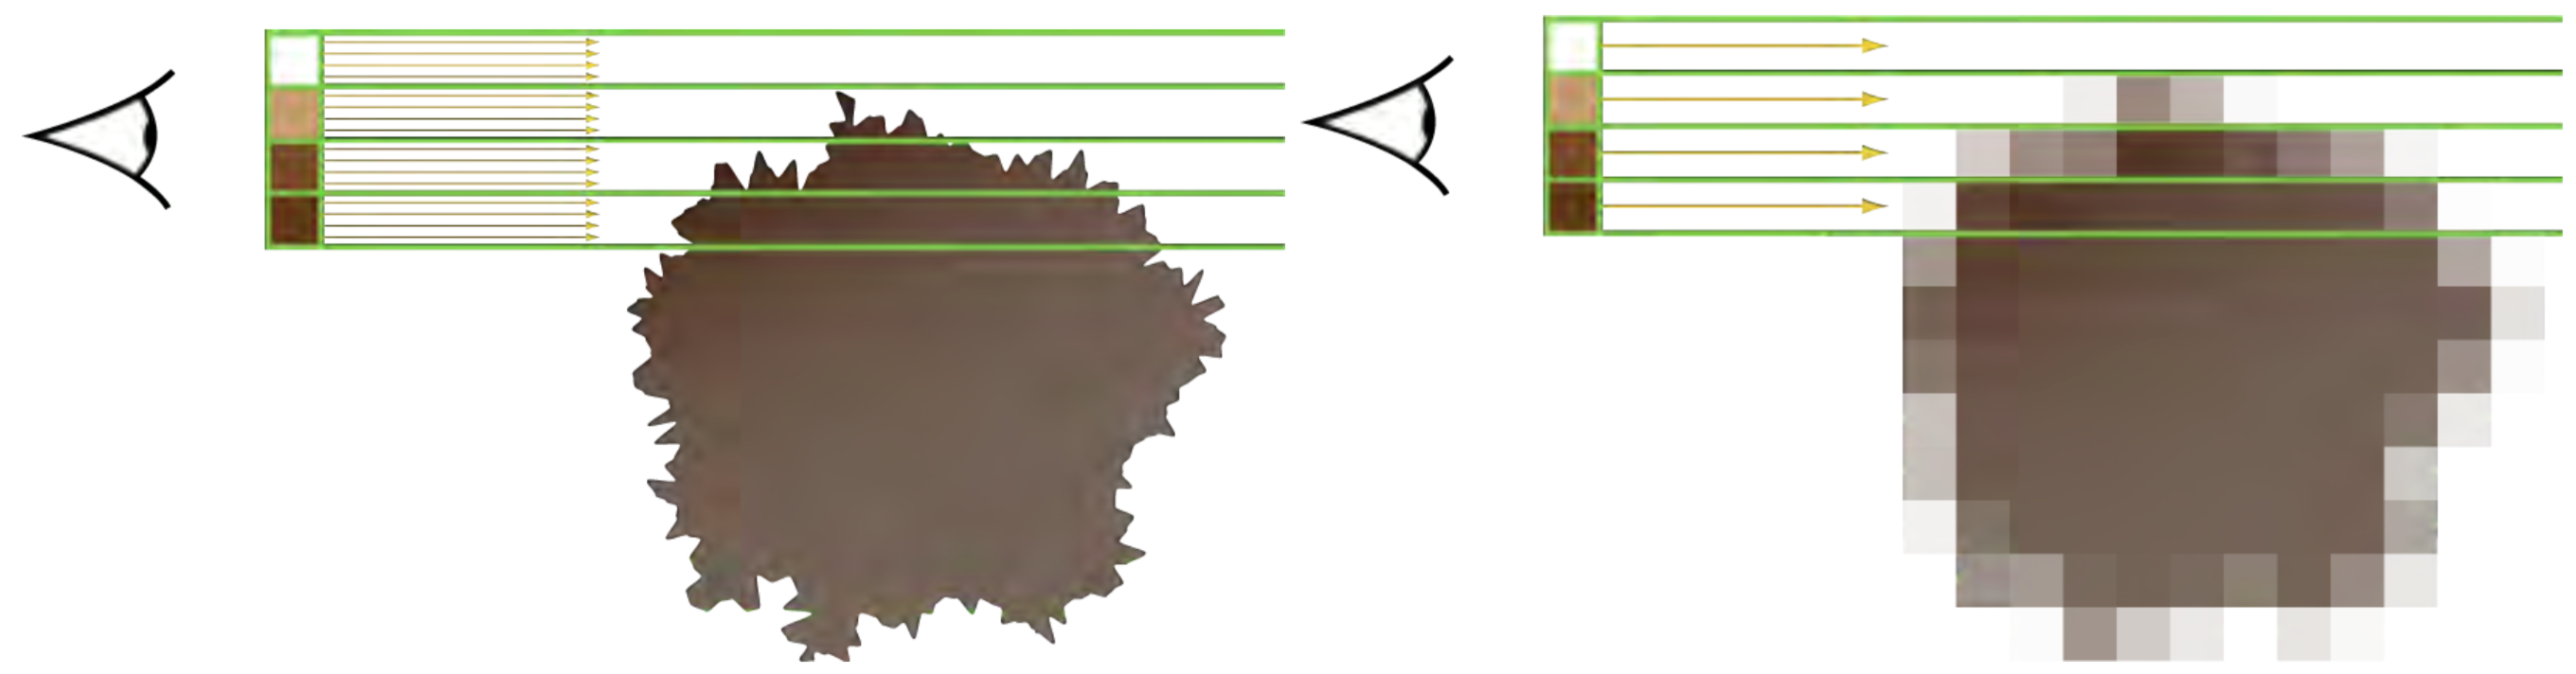
\includegraphics{graphics/vct/vct-4-3}
		\caption{Ray tracing: many rays}
	\end{subfigure}
	\caption{Left: Illustration of an highly detailed object rendered (through 4 pixels) with adaptive multisampling (left) and voxel-based pre-filtering (right)}
\end{figure}

Multi-resolution representations are easily obtainable based on MIP-mipping of voxel grids, making output-sensitive results possible. In figure \ref{f:vct-voxel-based-pre-filtering}, voxel MIP-mapping with inner-levels interpolation allows exactly adapting the geometrical resolution to the screen resolution.




\subsection{Pre-integrated Cone Tracing}
While classical boundary representation (B-rep) surface definitions can not be linearly combined, we replace them by a statistical distribution of densities stored as voxels into a regular subdivision of space, that we can be linearly pre-filtered inside a MIP-map pyramid, as explained in the previous section.

In our context, we want to store filtered material and geometry information at multiple scales, that will allow a quick rendering of very-complex geometry, and to dynamically compute the light interaction at all scales during rendering. Typically, we want at least a filtered density (or an opacity based on the density), a material color and a normal information per voxel.

Since first discussed by Crow\cite{a:Thealiasingproblemincomputer-generatedshadedimages} in the middle of 1970s, aliasing has been a major problem in rendering. One screen pixel is associated with more than just a line in space. It actually corresponds to a cone because a pixel covers an area and not a single point on the screen (as illustrated in figure \ref{f:vct-aliasing}). The is typically the source of aliasing that arises when a single ray is used per-pixel to sample the scene.

\begin{figure}\label{f:vct-aliasing}
	\begin{center}
		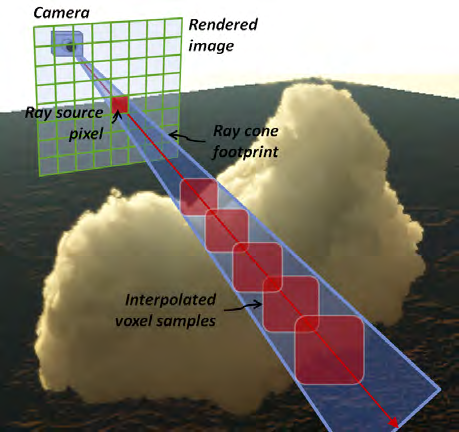
\includegraphics[width=0.6\textwidth]{graphics/vct/vct-6-1}
	\end{center}
	\caption{Illustration of the cone-shaped beam of light generated by the perspective projection and going toward a given pixel. We approximate it using a single ray launched from the pixel and sampling a pre-integrated representation of the scene geometry.}
\end{figure}

In order to integrate the incident radiance coming from a cone footprint, one needs to integrate the incoming radiance $I(D,\omega)$ from all $\omega$ directions in the cone:

\begin{equation*}
	I=\int_\Omega I(D,\omega)d\omega
\end{equation*}

Classical supersampling approaches discretize this integral with multiple rays to deal with aliasing, which lead to a very costly evaluation. Other approaches like cone or beam tracing provide faster antialiasing, but rely on an analytical definition of the geometry and can not be applied in a general case. Instead, we propose a model that is based on a single ray per pixel, and deals with aliasing by relying on a pre-filtered geometry representation stored inside a MIP-map pyramid.

This approximated cone tracing is done under the assumption that we can approximate the integration over a cone of visibilities, with the integration along a single ray of pre-integrated spatial visibilities. We base our mode upon the classical volume rendering integration model. In the next section, we will describe step by step how we build this pre-integrated rendering model, together with assumptions we make on the rendered data in order to allow it. 



\subsubsection{Volume Rendering}
Let's first take a look at volume rendering. The radiance along a light ray is affected when it passes through a participating medium. This interaction between light and matter is modelled as three different types of interactions: \textit{Emission, Absorption and Scattering} effects. \textit{Emission} describes the amount of radiative energy of light that is directly emitted by the participating media. \textit{Absorption} is the amount of energy that is absorbed by the material. Finally, \textit{Scattering} described the amount of energy that is scattered by the material, changing the direction of the propagation of the light. Scattering can both increase (in-scattering) and reduce (out scattering) radiative energy along a light ray.

Consider a parameter $s$ along a line segment expressed by $x=p+s\omega$, with $p$ being some arbitrary reference point, the equation of light transfer is:

\begin{equation*}
	\frac{dI(s)}{ds}=-\chi (s)I(s)+\eta (s)
\end{equation*}

where $\eta (s)$ is the total absorption coefficient, which is defined as the sum of $\kappa$, the true absorption coefficient, and $\sigma$ the \textit{out-scattering} coefficient: $\chi=\kappa+\sigma$. And the term $\eta(s)$ is the total emission coefficient that is the sum of the true emission coefficient $q$ and the \textit{in-scattering} coefficient $j$: $\eta=q+j$.

For the following work, we will concentrate on the \textit{emission-absorption} optical model, which neglects scattering and indirect illumination effects and represents only local light emission and absorption. Within this model, the equation of the light transfer reduces to:

\begin{equation*}
	\frac{dI(s)}{ds}=-\kappa (s)I(s)+q(s)
\end{equation*}

This integro-differential equation can be solved transformed into a pure integral equation by solving it along the direction of the ray between a starting point $s=s_0$ and an end point $s=D$, relative to back-to-front traversal. Boundary conditions also need to be fixed and we define $I_0$ the initial radiance along the ray at $s=s_0$. This leads to the \textit{volume rendering integral}\cite{b:Real-timeVolumeGraphics}:

\begin{equation*}
	I(D)=I_0 e^{-\tau (s_0,D)}+\int^{D}_{s_0}q(s)e^{-\tau (s,D)}ds
\end{equation*}

The term $\tau(s_1,s_2)$ is called the \textit{optical depth} or \textit{optical thickness} between position $s_1$ and $s_2$ and is defined as a measure of the proportion of radiation absorbed ot scattered along a path through a partially transparent medium. It is defined as:

\begin{equation*}
	\tau(s_1,s_2)=\int^{s_2}_{s_1}\kappa(t)dt
\end{equation*}

The corresponding transparency $T(s_1,s_2)$ (in [0,1]) is defined as:

\begin{equation*}
	T(s_1,s_2)=e^{-\tau(s_1,s_2)}
\end{equation*}

This leads to the following simplified version of the volume rendering integral:

\begin{equation*}
	I(D)=I_0T(s_0,D)+\int^{D}_{s_0}q(s)T(s,D)ds
\end{equation*}




\subsubsection{Volume Pre-integration Theory}
In our model, we consider the total absorption coefficient $\chi(s,r)$ on a point $s$ along a ray $r$. The participating medium represents a filtered geometry that rarely emits light on its own, but instead more often scatters (in the view direction) some energy coming from an external light source. Thus, we do not consider the true emission coefficient $q$. Instead, we consider the in-scattering coefficient $j(s,r)$ that corresponding to the energy reflected (scattered) by our filtered surface and material model on a point $s$ along a ray $r$ in the direction of the eye.

\begin{figure}\label{f:vct-pre-integration-1}
	\begin{center}
		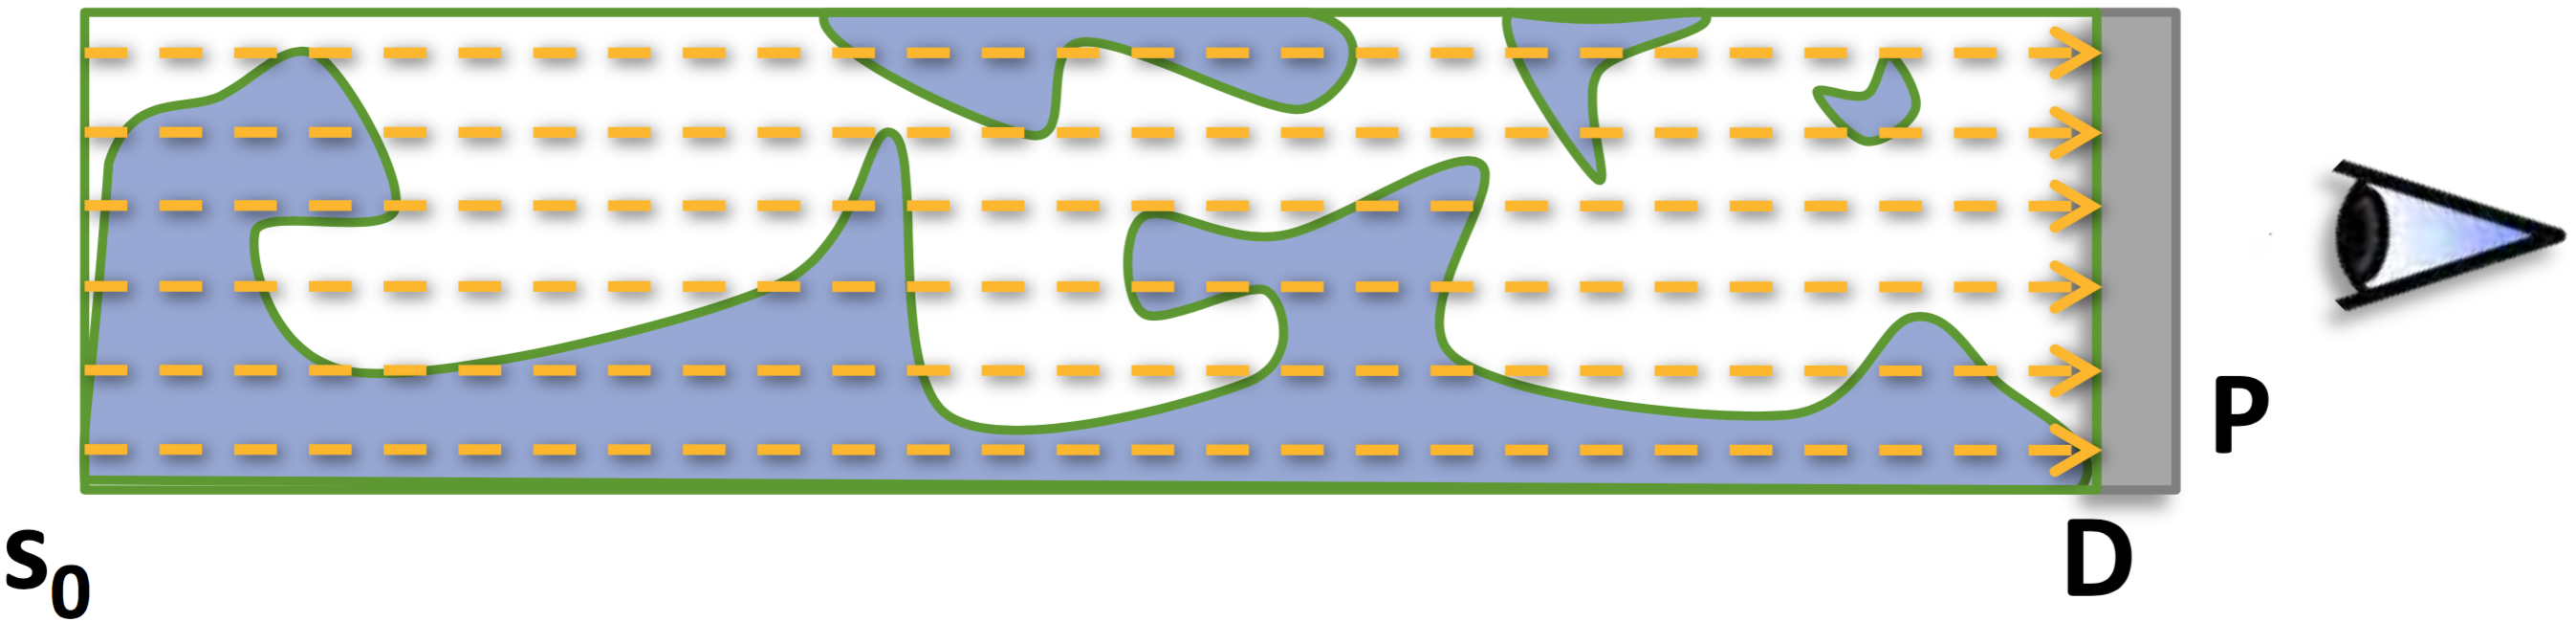
\includegraphics[width=0.9\textwidth]{graphics/vct/vct-7-1}
	\end{center}
	\caption{Integration over a pixel footprint of the volume rendering integration along orthographic rays.}
\end{figure}

In this explanation, we first assume a parallel projection leading to orthographic beams generated by pixel footprint, we'll see later how to extend this model to perspective projection with cone-shaped beams.



Our goal is to build a pre-integration model for the computation of the average energy $I(D,P)$ accumulated over the footprint of a pixel $P$ on the screen. This can be modelized as the integration of the volume rendering integral along a ray $r$ over the footprint of the pixel $P$ as described by equation \ref{eq:vct-1} and illustrated in figure \ref{f:vct-pre-integration-1}. 

\begin{equation}\label{eq:vct-1}
	I(D,P)=\int_{r\in P}\int^{D}_{s_0}j(s,r)e^{-\int^{D}_s\chi(t,r)dt}dsdr
\end{equation}

What we propose is to replace the integration over a pixel of the ray-based volume rendering integration function, by a pre-integration inside a set of cubical volumes of this function in object space as illustrated in figure \ref{f:vct-pre-integration-2}. Our goal is to store a discrete set of these pre-integrated volumes per-voxel inside a 3D MIP-map pyramid, in order to use them for fast rendering.

\begin{figure}\label{f:vct-pre-integration-2}
	\begin{center}
		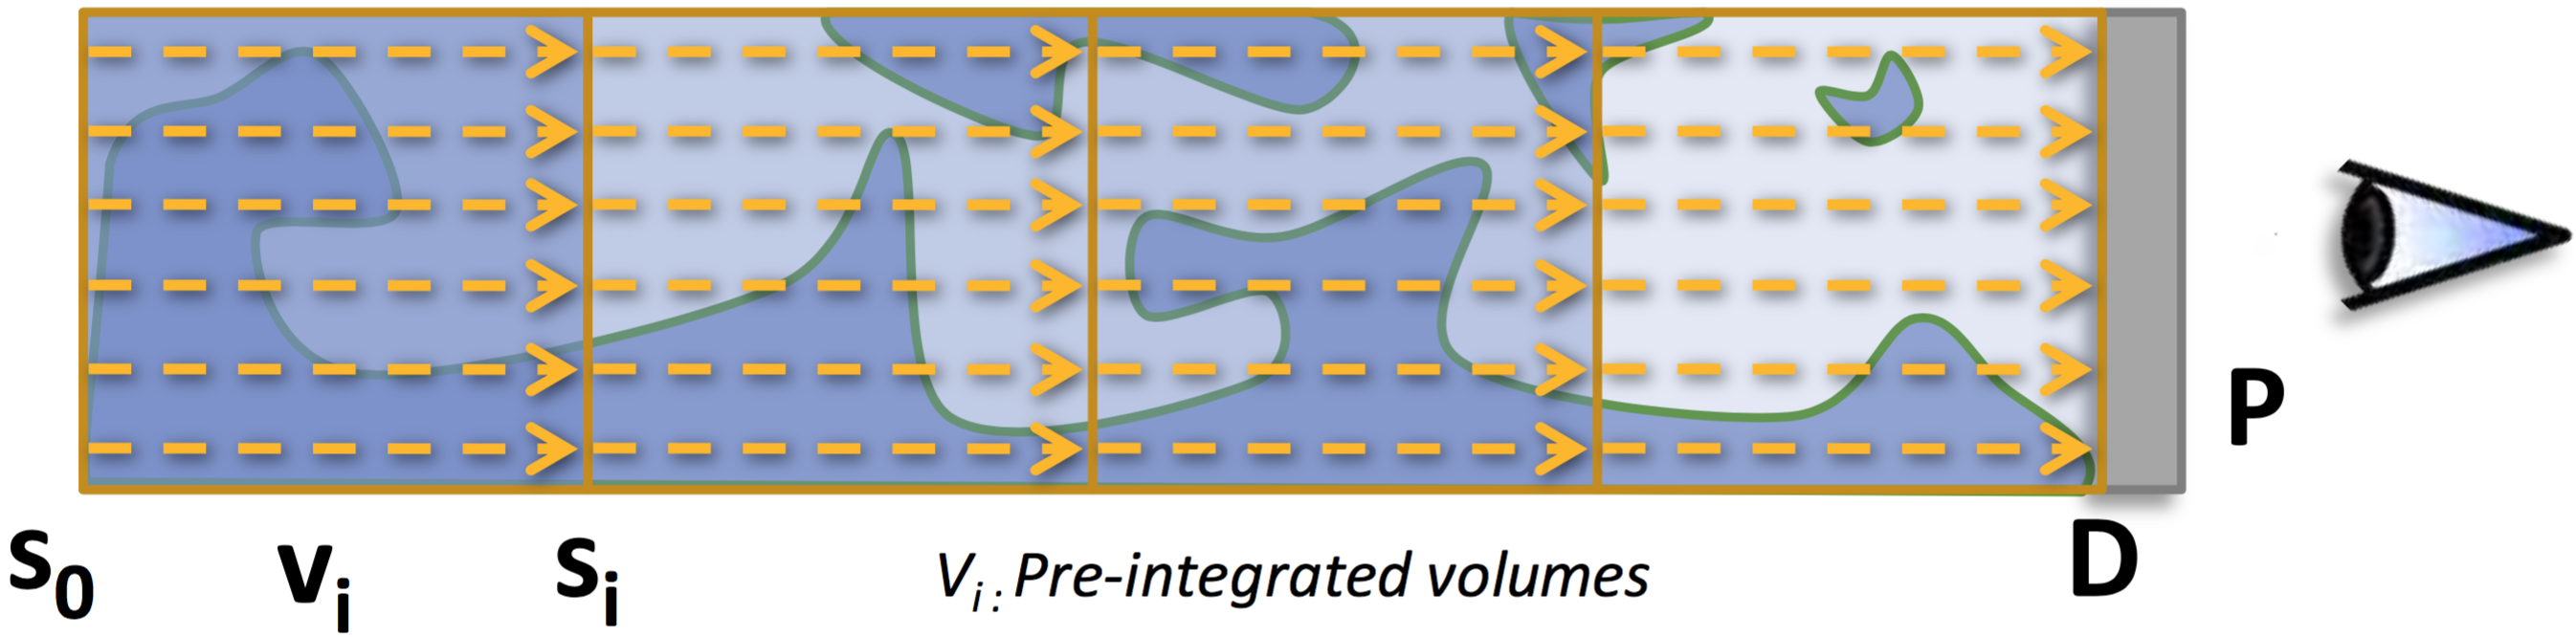
\includegraphics[width=0.9\textwidth]{graphics/vct/vct-7-2}
	\end{center}
	\caption{Accumulation for a pixel of the pre-computation inside sub-volumes of the volume integration.}
\end{figure}

First, we need to split the volume integration along a single ray into a discrete number of sub-integrations that can be precomputed. In order to simplify the equations, we denote $\tau(s_1,s_2),r$ the \textit{optical depth} that corresponds to a local path integration of the total extinction between $s_1$ and $s_2$ along a ray $r$:

\begin{equation*}
	\tau(s_1,s_2,r)=\int^{s_2}_{s_1}\chi(s,r)ds
\end{equation*}

And we denote $Q(s_1,s_2,r)$ the local path integration of the in-scattering energy:

\begin{equation*}
	Q(s_1,s_2,r)=\int^{s_2}_{s_1}j(s,r)e^{-\tau(s,s_2,r)}ds
\end{equation*}

Based on these notations, we split the integration along rays on the interval $[s_0,D]$ into a discrete number of local sub-paths $[s_i,s_{i+1}]$, for both the energy integration part and the sub-integration of the attenuation:

\begin{equation*}
	I(D,P)=\int_{r\in P}\sum^{n}_{i=0}(Q(s_i,s_{i+1},r)\cdot e^{-\sum^{n}_{j=i+1}\tau(s_j,s_{j+1},r)})dr
\end{equation*}

These discrete summations correspond to the marching process done along rays in classical ray-casting rendering approaches.

According to the Fubini's theorem\sidenote{\url{http://mathworld.wolfram.com/FubiniTheorem.html}}, based on the continuity of all functions (all parameters are defined continuously in space), we can swap the discrete sum and the integration over the whole expression:

\begin{equation*}
	I(D,P)=\sum^{n}_{i=0}\Bigg( \int_{r\in P}Q(s_i,s_{i+1},r)\cdot e^{-\sum^{n}_{j=i+1}\tau(s_j,s_{j+1},r)}dr\Bigg)
\end{equation*}

We will now use a general hypothesis on our data: on a given ray $r$, a sub-path integration of energy $Q(s_i,s_{i+1},r)$ is decorrelated from $e^{-\sum^{n}_{j=i+1}\tau(s_j,s_{j+1},r)}$, the integration of the total absorption happening on the whole path between $s_{i+1}$ and the position of the eye. This means that these two values do not have a statistical dependence. Within this hypothesis, thanks to the definition of the statistical correlation $correlation(a(),b())=\int a()b()-\int a()\int b()$, we can replace the integral of the product of the two decorrelated terms by the product of their integral:

\begin{equation*}
	I(D,P)\approx \sum^{n}_{i=0}\Bigg(\Bigg( \int_{r\in P}Q(s_i,s_{i+1},r)dr\Bigg)\cdot\Bigg( \int_{r\in P} e^{-\sum^{n}_{j=i+1}\tau(s_j,s_{j+1},r)}dr\Bigg)\Bigg)
\end{equation*}

Thanks to this hypothesis, we already obtain a formulation of the in-scattered energy in the form we were looking for, pre-integrated over a pixel $P$ between the parameters $s_1$ and $s_2$: $\overline{Q}(s_1,s_2,P)=\int_{r\in P}Q(s_1,s_2,r)dr$

We now need to get a similar expression for the pre-integration of the optical depth. To do so, we need to bring the integration over $P$ inside the inner sum of optical depths computed in the exponential. Instead of trying to pull the integration over $P$ up in the exponential, we pull down the sum from the exponential into a product of exponentials:

\begin{equation*}
	I(D,P)\approx \sum^{n}_{i=0}\Bigg(\Bigg( \int_{r\in P}Q(s_i,s_{i+1},r)dr\Bigg)\cdot\Bigg( \int_{r\in P}\prod^{n}_{j=i+1} e^{-\tau(s_j,s_{j+1},r)}dr\Bigg)\Bigg)
\end{equation*}

In fact, this formulation as a product of exponentials corresponds exactly to the way transparency $T(s_1,s_2,r)=e^{-\tau(s_1,s_2,r)}$ is classically computed with a discrete integration on a given path along a ray. Thus, we chose to pre-integrate transparency instead of the optical depth itself. With this formulation, the only operation remaining in order to get a formulation of the pre-integrated transparency is to swap the integral over $P$ and the product operator.

Once again, we rely on a correlation hypothesis, we can swap the integral over $P$ and the product operator:

\begin{equation*}
	I(D,P)\approx \sum^{n}_{i=0}\Bigg(\Bigg( \int_{r\in P}Q(s_i,s_{i+1},r)dr\Bigg)\cdot\prod^{n}_{j=i+1}\Bigg( \int_{r\in P} e^{-\tau(s_j,s_{j+1},r)}dr\Bigg)\Bigg)
\end{equation*}

We now get the two functions we want to pre-compute and store in our pre-integrated voxel representation, the average in-scattered energy $\overline{Q}$ and average transparency $\overline{T}$: 

\begin{equation*}
	\begin{aligned}
		\overline{Q}(s_1,s_2,P)=&\int_{r\in P}Q(s_1,s_2,r)dr\\
		\overline{T}(s_1,s_2,P)=&\int_{r\in P}e^{-\tau(s_1,s_2,r)}dr
	\end{aligned}
\end{equation*}

That leads us to the following render-time integration scheme that will be implemented by rendering algorithm presented in the next sections:

\begin{equation}\label{eq:vct-2}
	I(D,P)\approx \sum^{n}_{i=0}\Bigg(\bigg( \overline{Q}(s_1,s_2,P)\bigg)\cdot\prod^{n}_{j=i+1}\bigg( \overline{T}(s_1,s_2,P)\bigg)\Bigg)
\end{equation}




\subsubsection{Discrete Composition Scheme}
Thanks to the model we just presented, and based on equation \ref{eq:vct-2}, it is possible to evaluate the radiative light $I(D,P)$ coming from a beam, towards a pixel $P$, by sampling along a single ray.

To do so, we define a composition scheme that can be used to incrementally compute $I(D,P)$. For a pixel $P$, we define $\overline{Q}_i=\overline{Q}(s_i,s_{i+1},P)$ and $\overline{T}_i=\overline{T}(s_i,s_{i+1},P)$, as well as accumulated energy $\hat{I}_i$ at position $i$ and transparency $\hat{T}_i$. This leads to the following front to back compositing scheme, with the final $I(D,P)=\hat{I}_0$:

\begin{equation*}
\begin{aligned}
	\hat{I}_i=&\hat{I}_{i+1}+\hat{T}_{i+1}\overline{Q}_i\\
	\hat{T}_i=&\hat{T}_{i+1}\overline{T}_i
\end{aligned}
\end{equation*}

with the initialization: $\hat{I}_n=\overline{Q}_n$ and $\hat{T}_n=\overline{T}_n$.




\subsubsection{World-space Definition}
Based on the model we just described that is expressed in ray-space, we want to pre-compute the two functions $\overline{Q}$ and $\overline{T}$ in world-space, so that they can be stored per-voxel in our MIP-map representation. Thus, we redefine these two functions depending on a position $\mathbf{p}$, a direction $\mathbf{d}$, a surface area of integration $s$ and a length $l$:

\begin{equation*}
	\begin{aligned}
		\overline{Q}(\mathbf{p},\mathbf{d},s,l)=&\int_{r\in (s,p,d)}Q(s,s+l,r)dr\\
		\overline{T}(\mathbf{p},\mathbf{d},s,l)=&\int_{r\in (s,p,d)}e^{-\tau(s,s+l,r)}dr
	\end{aligned}
\end{equation*} 

We will see in the next section how we discretize and store these 8D functions inside our voxel MIP-map pyramid. 




\subsection{MIP-map Pre-integration Model}\label{sec:mip-map-pre-integration-model}
\begin{marginfigure}
	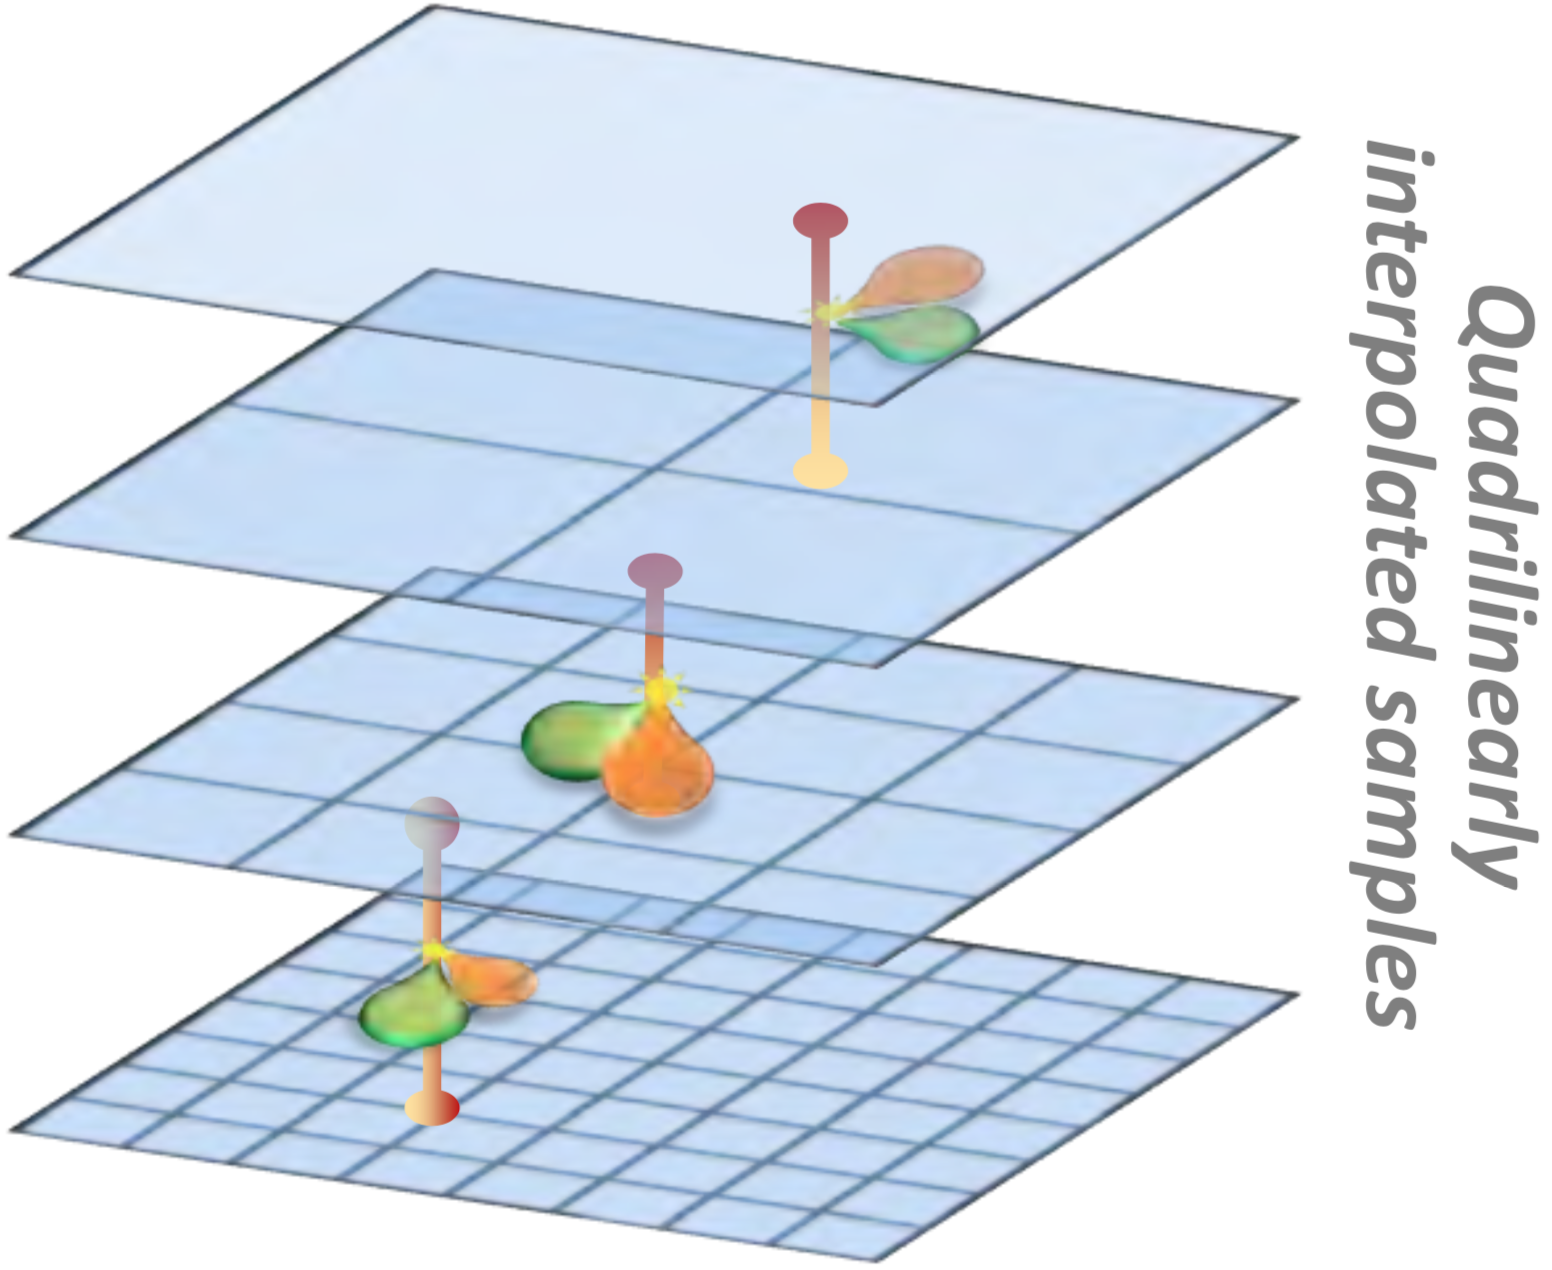
\includegraphics{graphics/vct/vct-7-6}
	\caption{Mipmap pyramid of pre-integrated values.}
	\label{f:vct-mipmap-pyramid}
\end{marginfigure}

Our goal is to discretize our pre-integrated energy function $\overline{Q}(\mathbf{p},\mathbf{d},s,l)$ and pre-integrated transparency function $\overline{T}(\mathbf{p},\mathbf{d},s,l)$ for non-overlapping cubical volumes stored in a set of regular voxel grids of decreasing resolutions organized as a 3D MIP-map pyramid (see figure \ref{f:vct-mipmap-pyramid}). Thus, we want to pre-compute these functions for a discrete set of positions $\mathbf{p}$ regularly distributed in space, and a set of length of integration $l$ corresponding to the size of the voxel, and thus determining the level in pyramid. As we want to maintain cubical voxels, we link this length of integration $l$ to the surface area parameter $s$ that we re-compute for square areas $s=l^{2}$. Thus, the pre-computation over large pixel integration footprints leads to long pre-integrated lengths, but this allows a storage inside a cubical voxels and provides a multi-resolution scheme.

\begin{figure}\label{f:vct-pre-integration-3}
	\begin{center}
		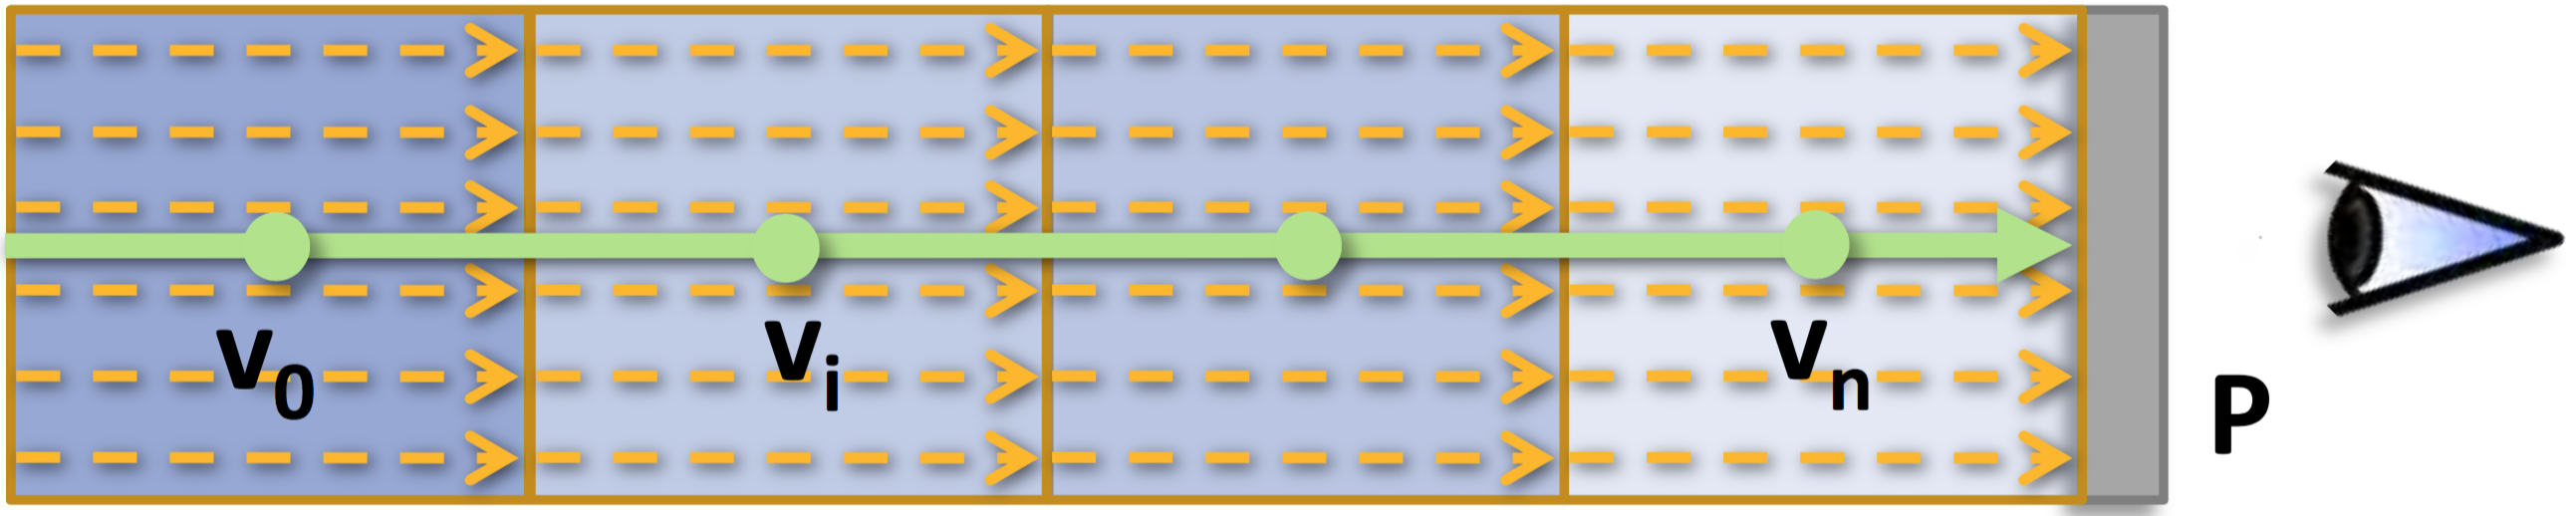
\includegraphics[width=0.9\textwidth]{graphics/vct/vct-7-3}
	\end{center}
	\caption{Accumulation along a single ray launched for given pixel of the pre-integrated sub-volumes stored inside the MIP-map pyramid. $V_i$: Pre-integrated volumes.}
\end{figure}

The pre-integrated transparency $\overline{T}$ stored per-voxel in our volumetric representation corresponds to the transparency of the volume when seen through a section that has the same size is the voxel it is stored in. Similarly, the pre-integrated in-scattered energy $\overline{Q}$ corresponds to the energy added along a ray by the filtered materials represented inside a voxel. We will see that in practice, we do not want to pre-integrate and store $\overline{Q}$ directly per voxel, but instead we want to store the shading parameters allowing to dynamically compute $\overline{Q}$ at render time.

With this representation, the only parameter remaining per voxel to fully represent $\overline{Q}(\mathbf{p},\mathbf{d},s,l)$ and $\overline{T}(\mathbf{p},\mathbf{d},s,l)$ is the direction of integration $\mathbf{d}$.



\subsubsection{Quadrilinear Interpolation}
At render time, one ray is launched per pixel of the screen. Values are sampled along this ray inside the MIP-map pyramid, at a level-of-detail (LOD) chosen in order to get a pre-integrated surface $s$ corresponding to the pixel size. Values for continuous volume positions $\mathbf{p}$ and continuous footprint area $s$  are reconstructed by interpolation of the values stored inside the MIP-map pyramid. 

We first discuss the interpolation inside a given MIP-map level in order to reconstruct values at continuous positions. If we consider a single ray, the pre-integrated transparency $T$ does involve bilinearly on the plane orthogonal to the ray (parallel to the screen), and thus can be bilinearly interpolated on this plane. However, this pre-integrated transparency $\overline{T}$ does not evolve linearly in the direction of the ray. In this direction, the transparency evolves exponentially due to the volume rendering integration, and thus can not be linearly interpolated\sidenote{The same linear interpolability issue applies to the in-scattered energy $\overline{Q}$ that can be linearly interpolated orthogonally to a ray, but do not in the direction of the ray due to the visibility integration in this direction.}. Since we don't want to use a totally custom interpolation scheme (to benefit from the hardware trilinear texture interpolation), we rely on a linear interpolation in all axes. In practice, the impact on the rendering precision of this approximation appeared to be negligible in most cases.

The remaining interpolation is the one that needs to be done between two MIP-map levels, in order to reconstruct a continuous surface of integration s (since LOD footprints are quantified), and linked length of integration $l$. Transparency evolves exponentially with the length of integration $l$. Thus, since both $\overline{Q}$ and $\overline{T}$ contain a transparency value, these values do not evolve linearly between two MIP-map levels. However, we chose to interpolate them linearly, once again for efficiency reasons, and given the low impact on rendering quality in most cases.





\subsubsection{Cone-shaped Beams}
As presented so far, our pre-integration model only allows the evaluation of the volume rendering integral inside orthographic beams generated by a parallel projection. We will now explain how we rely on the MIP-map pyramid representation detailed in the previous section and storing our pre-integrated energy and visibility functions to approximate cone-shaped beams generated by perspective projection.

\begin{figure}
	\begin{center}
		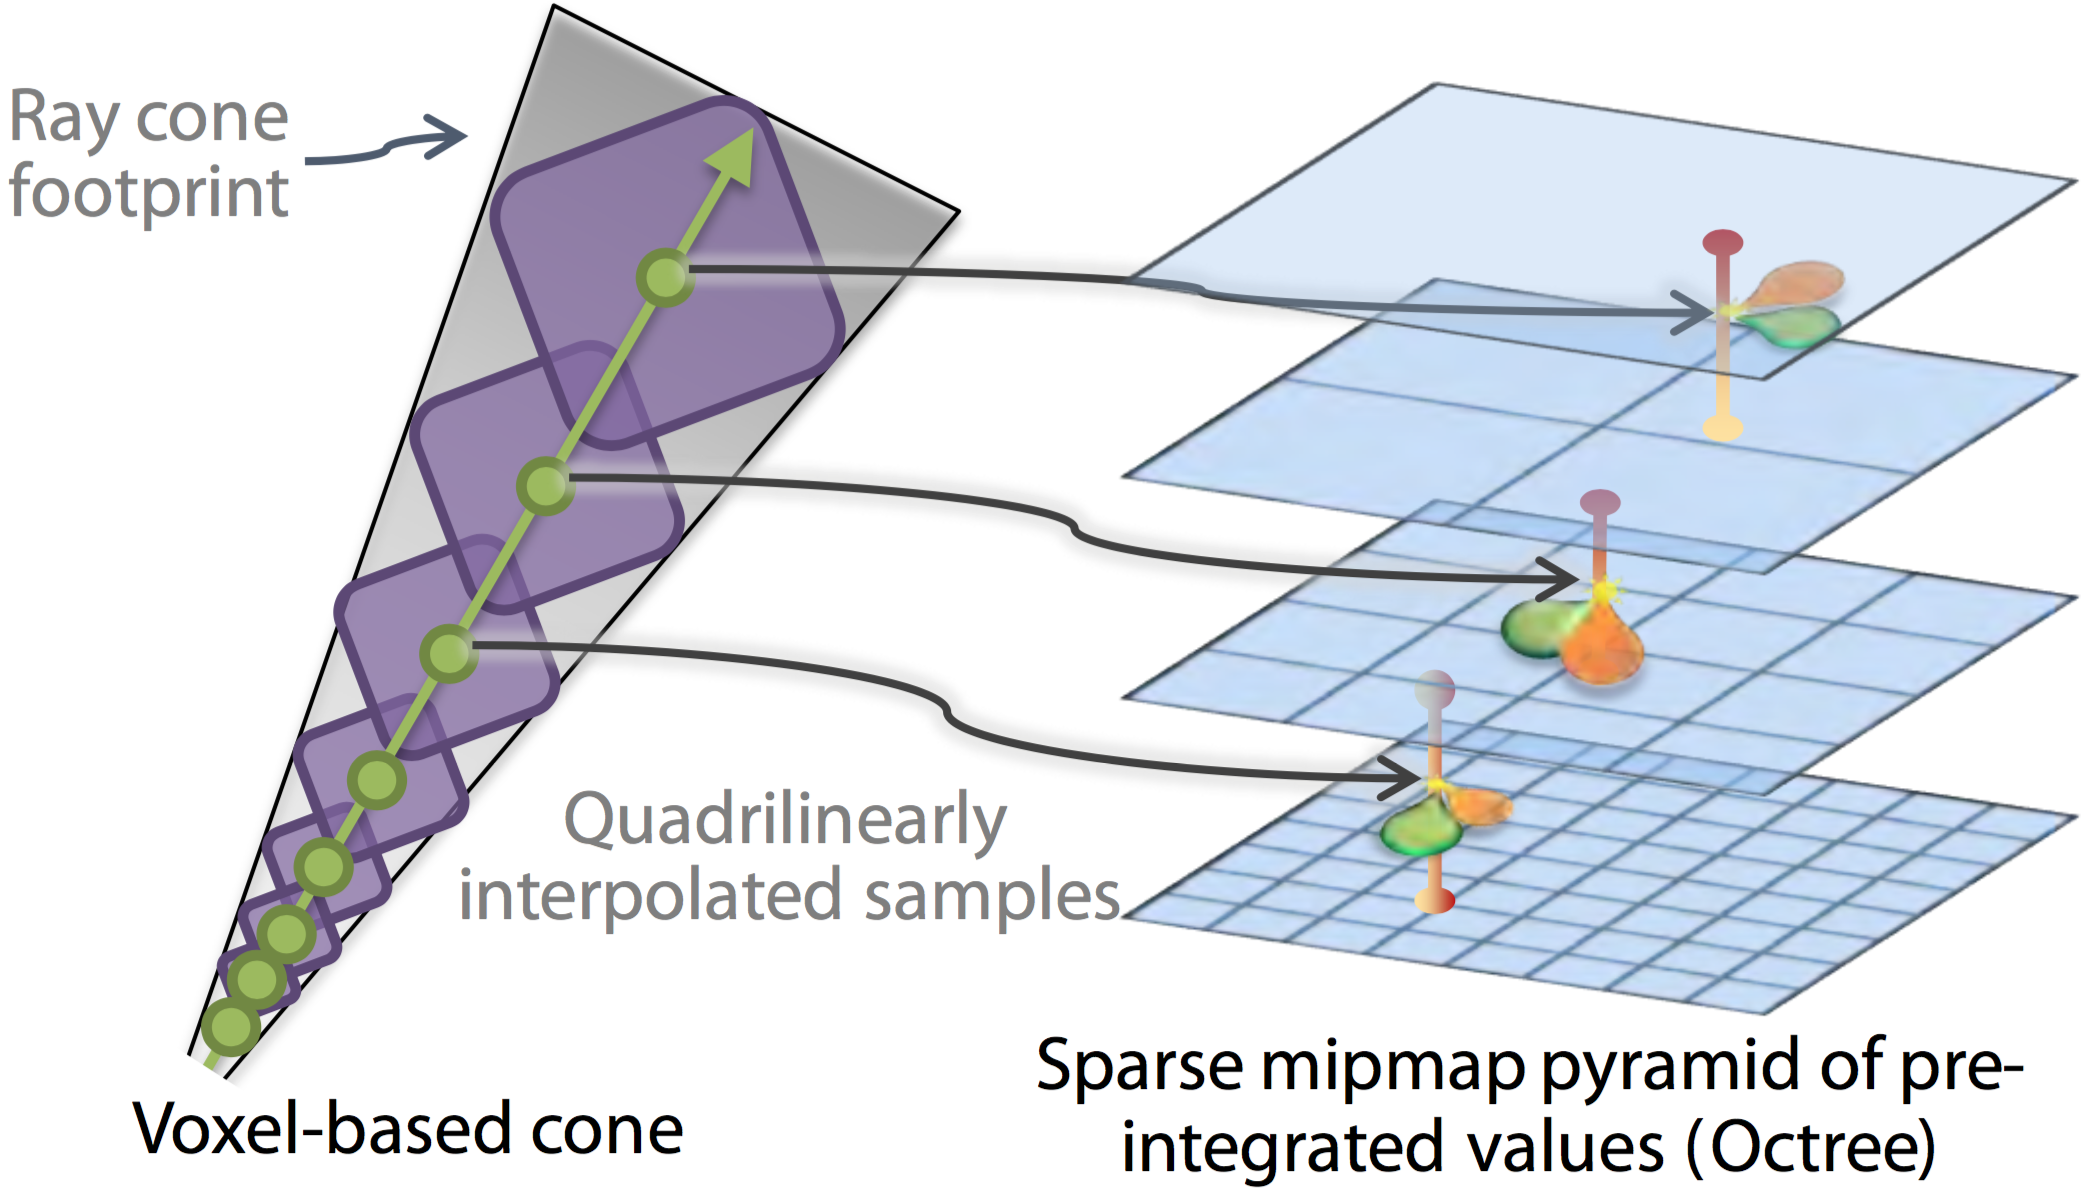
\includegraphics[width=0.75\textwidth]{graphics/vct/vct-7-4}
	\end{center}
	\caption{Illustration of one ray sampling using quadrilinear interpolation in the voxel mipmap pyramid.}
\end{figure}

In practice, for anti-aliasing, we rely on very thin cone (generated for each pixel) that can be considered as locally cylindrical. We approximate cone-shaped beams by simply varying the LOD used in the MIP-map pyramid when sampling along a ray\sidenote{But for a big cone, it leaves us with undersampling. We will talk about this in cascaded voxel cone tracing.}. The idea is, for each sample, to use the LOD providing the surface of integration $s$ approximating the section of the cone at the point where the sample is taken. The scheme is illustrated in figure \ref{f:vct-pre-integration-5}. As we have seen in the previous section, interpolation must be used between the values stored for discrete area $s$ in the levels of the MIP-map pyramid, in order to get the exact area required for each sample.

\begin{figure}\label{f:vct-pre-integration-5}
	\begin{center}
		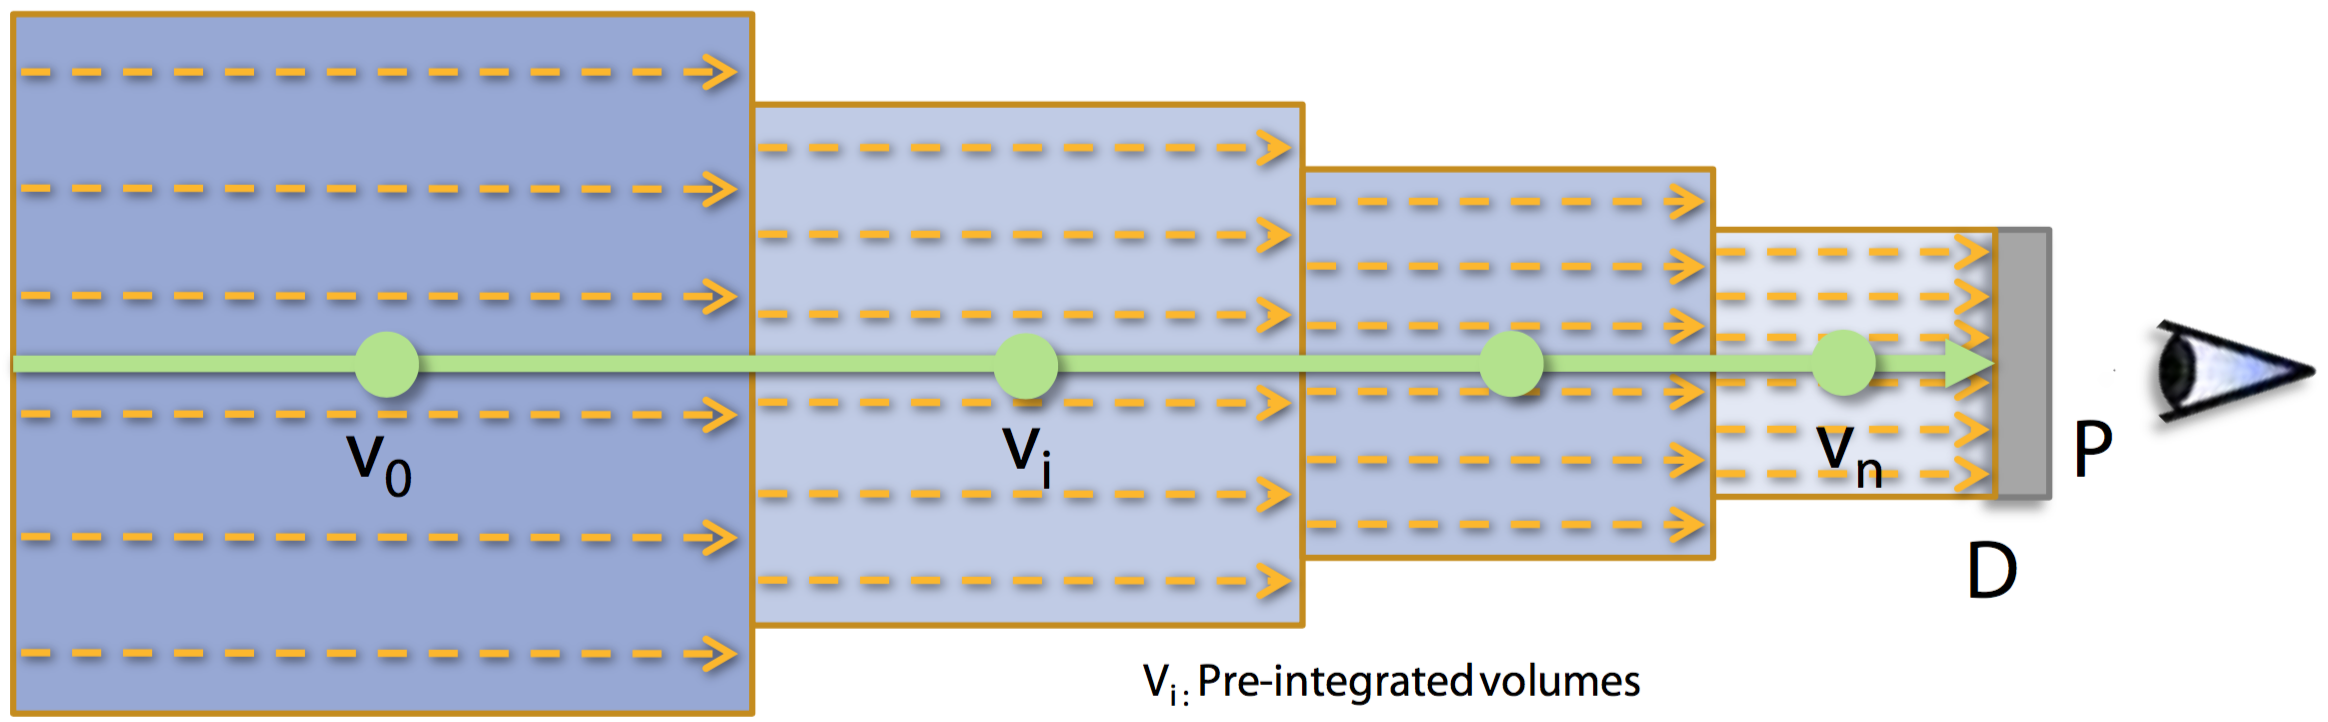
\includegraphics[width=0.9\textwidth]{graphics/vct/vct-7-5}
	\end{center}
	\caption{Illustration of a cone shaped beam approximated using our voxel-based cubical pre-integration. It is computed efficiently using only a few samples taken along a single ray.}
\end{figure}

As illustrated in figure \ref{f:vct-pre-integration-5}, the local projection inside pre-integrated sub-volumes corresponds to an orthographic projection, and not a perspective projection as would be expected. This simplification leads to a parallax not taken into account locally in each beam part. This error increases as the size of the pre-integrated volumes increases. In our typical case using thine cones for antialiasing, the small parallax error that can appears inside sub-volumes integrations can be considered as negligible. However, this error increases as much as the aperture of the cones increases.



\subsubsection{Cone Footprints}
The second approximation we make with our approach is to approximate the cone footprint, with cubically shaped sub-volumes aligned with the main axis of our MIP-map representation, as illustrated in figure \ref{f:vct-pre-integration-5}. The first thing to note is that we consider the cone footprint because we represent pixels as disks-shaped elements in order to simplify the representation.

\begin{figure}\label{f:vct-cone-footprints}
	\begin{subfigure}[b]{0.24\textwidth}
		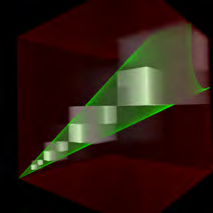
\includegraphics{graphics/vct/vct-8-1}
		\caption{}
	\end{subfigure}
	\begin{subfigure}[b]{0.24\textwidth}
		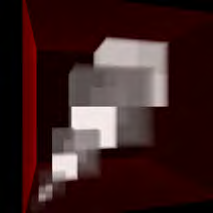
\includegraphics{graphics/vct/vct-8-2}
		\caption{}
	\end{subfigure}
	\begin{subfigure}[b]{0.24\textwidth}
		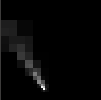
\includegraphics{graphics/vct/vct-8-3}
		\caption{}
	\end{subfigure}
	\begin{subfigure}[b]{0.24\textwidth}
		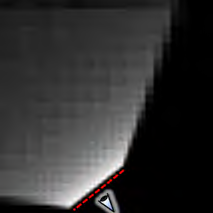
\includegraphics{graphics/vct/vct-8-4}
		\caption{}
	\end{subfigure}
	\caption{Display of the footprint of pre-integrated voxel cones, in 3D inside a volume (a, b) and inside a single slice of a volume for a single ray (c) and for a set of rays launched on a whole line of pixels (d).}
\end{figure}

Since values read in the MIP-map pyramid are interpolated both spatially and in resolution between MIP-map levels, the exact footprint of a cone inside the voxel representation is not trivial to estimate. In order to get an idea of this footprint, we display in figure \ref{f:vct-cone-footprints} the relative accumulated weight of each voxel (splatted inside the maximum resolution of the MIP-map pyramid) in the quadrilinear interpolation that is done each time they are accessed.

Figure \ref{f:vct-cone-footprints}(a) presents these weights inside a volume rendered in 3D for a cone aperture of $11.25^{\circ}$, and figure \ref{f:vct-cone-footprints}(b) for an aperture of $22.5\circ$. The same experiment is presented for a 2D cut inside a volume in figure \ref{f:vct-cone-footprints}(c). Even if the footprint of a single cone appears blocky, it in fact approximates a Gaussian distribution centered around the sampling ray. Thus, this approximation converges on a good quality sampling when multiple beams are sent from neighboring pixels. In deed, sampling a volume with such cones in fact globally ensures energy-conservation. This is illustrated in figure \ref{f:vct-cone-footprints}(d) that presents the same experiment for a set of rays launched on an entire line of pixels. One can observe that pixels appear regularly sampled, with a weight depending only on their distance to the screen (as expected).




\subsection{Pre-filtering Shading Parameters}
This model as described thus far assumed that the reflected energy $j$ was entirely known before rendering, and we stored its pre-integrated value $\overline{Q}$ in the pre-computed MIP-map representation. In order to allow fully dynamic lighting computation, we will now explain how it is possible to factor the lighting computation out of the pre-integration of $j$ inside $\overline{Q}$, and to pre-integrate only material parameters.

\begin{figure}\label{f:vct-local-shading-model}
	\begin{center}
		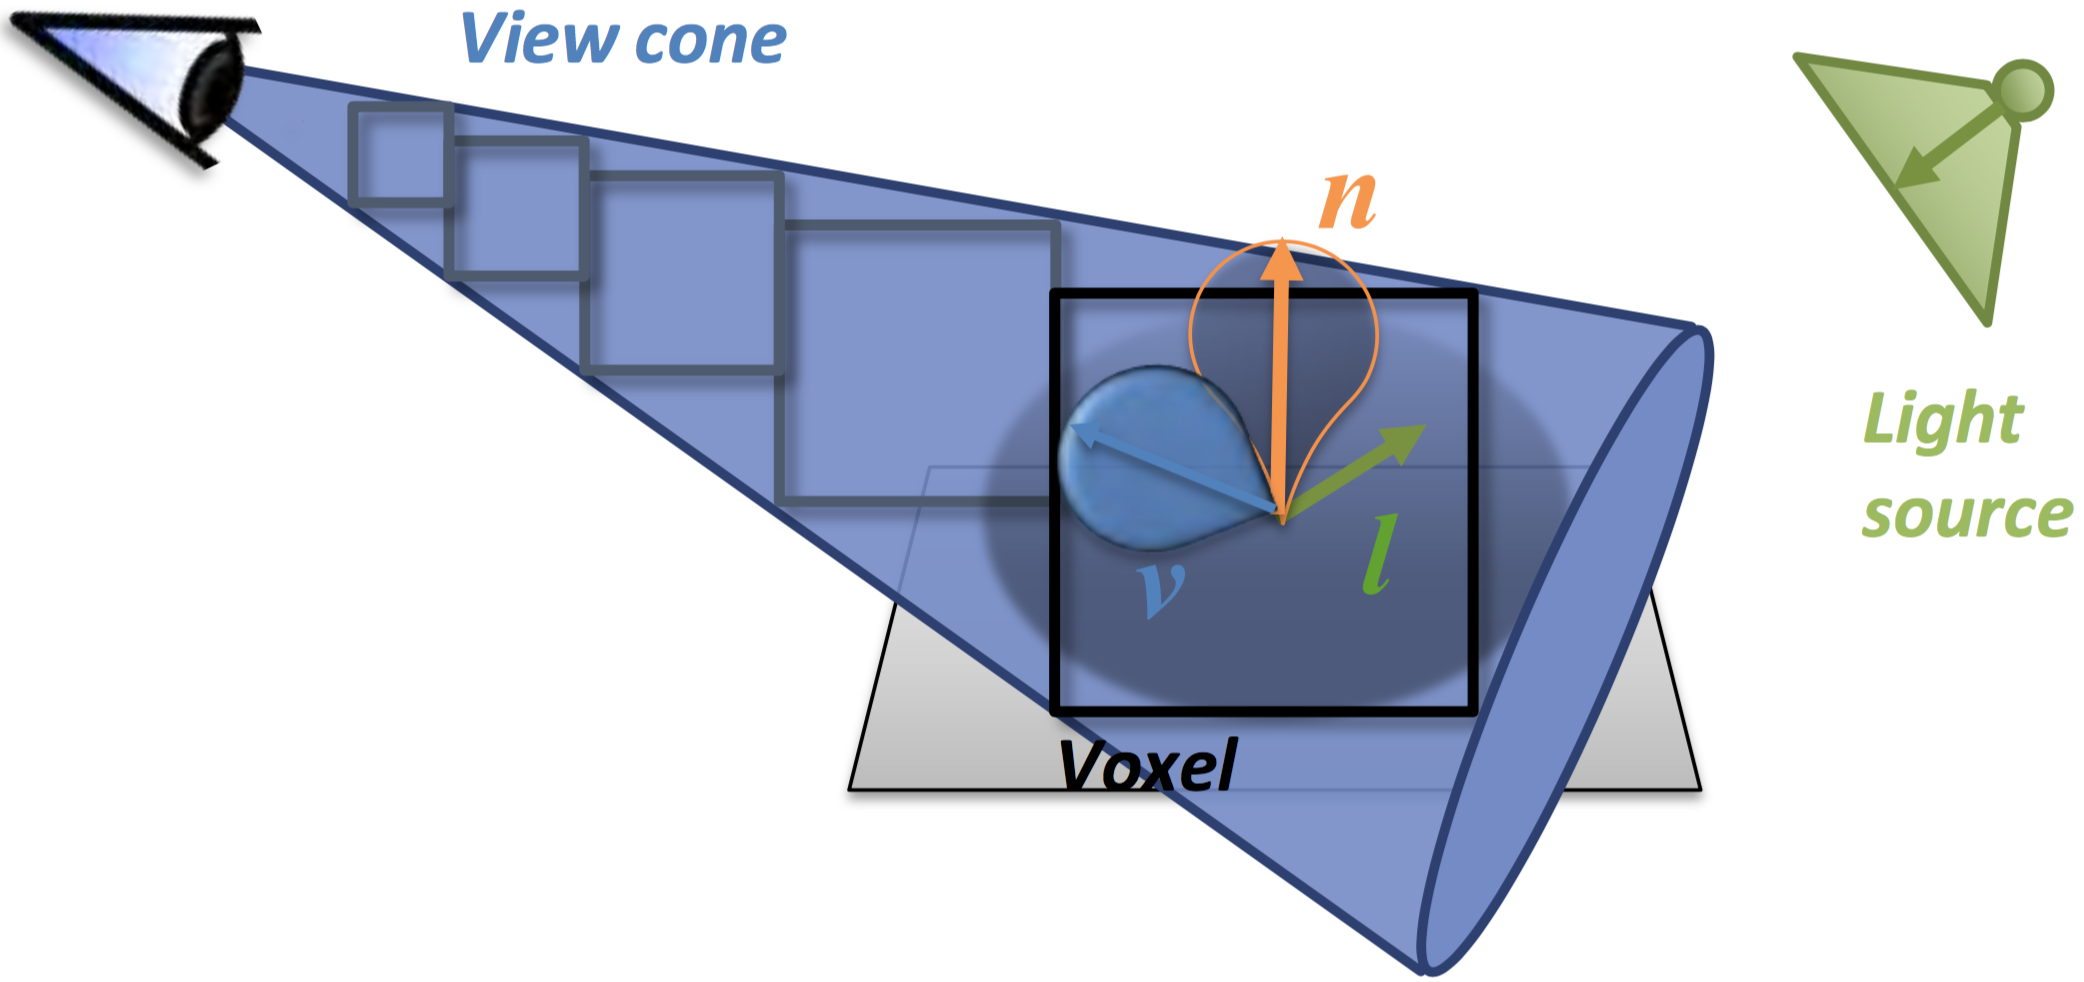
\includegraphics[width=0.6\textwidth]{graphics/vct/vct-9-1}
	\end{center}
	\caption{Illustration of our local shading model based on pre-filtered surface and material parameters.}
\end{figure}

Each voxel at a given LOD of the pre-integrated MIP-map pyramid must represent the light behavior of the lower levels -- and thus, of the whole span it represents. As we have known, texture pre-filtering techniques rely on the fact that, under some linearity assumptions, it is possible to factor-out from the shading integration some shading parameters and to pre-filter them separately in order to produce antialiased rendering. This operation is possible only when the shading parameters that are factored-out have a linear relationship to the final color, meaning they are involved only linearly in the shading function.



\subsubsection{Material Parameters}
This simple model we used is based on a single vector of material colors $C_{RGB}$, a surface normal $N$ and a global analytical BRDF (Phone). Since the material color has a linear relationship to the final color in the shading computation, it can be freely factored-out and pre-integrated separately. We store a vector of pre-integrated color values $\overline{C}_{RGB}$ for each voxel of out representation and filter it during the MIP-map construction described in the next section. 

Things are more difficult concerning the normals, a simple vector-based normal description can not be linearly filtered. Thus, we rely on a normal distribution function stored per-voxel and representing the filtered distribution of surface normals in a given volume.



\subsubsection{Simple Normal Distribution}
While the material color can be freely pre-integrated, it is not the case for the surface normal information $N$ that is needed to compute a local shading model. Filtering normal map representations has been a long studied problem. Normal map filtering approaches are based on the idea of representing the normal information using a statistical distribution of normal directions over a surface (called \textit{normal distribution function}, NDF), that can be linearly filtered. Accurate NDF representations (based on spherical harmonics for instance) have been proposed in the past. While such representations are totally allowed by our model and are required for a high degree of filtering (when many objects are aggregated), we considered them too memory-intensive for moderate filtering. Instead in our examples, we choose to store only isotropic Gaussian lobes characterized by an average vector $D$ and a standard deviation $\sigma$ as proposed by Toskvig\cite{a:Mipmappingnormalmaps}. In order to ease the pre-filtering (computation of the MIP-map pyramid) and interpolation, the variance is encoded via the norm $|D|$ such that $\sigma^{2}=\frac{1-|D|}{|D|}$. This representation supposes an anisotropic sub-geometry distribution, a moderate filtering and a single filtered face pre-voxel.



\subsubsection{Local Shading Model}
At render time, the actual pre-integrated in-scattered energy $\overline{Q}$ is computed for each sample taken inside the voxel representation. This computation is done by applying a local shading model (in our examples a simple Phone), based on the vector of material colors $\overline{C}_{RGB}$, the filtered normal distribution (NDF) $\overline{N}$ and the directions to the eye, and to the point light source.

For this, we have to account for the variations in the embedded directions and scalar attributes. For relatively large cone apertures, the span of the cone that is currently accumulating the current voxel must also be taken into account as illustrated in figure \ref{f:vct-local-shading-model-1}. This can conveniently be translated into convolutions, provided that the elements are decomposed into lobe shapes. In our case, we have to convolve the NDF, the BRDF and the span of the view cone, the first already being represented as Gaussian lobes.

\begin{figure}\label{f:vct-local-shading-model-1}
	\begin{center}
		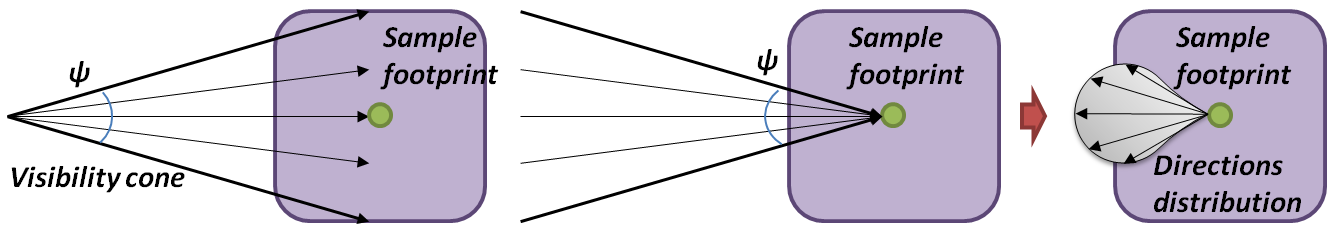
\includegraphics[width=1.\textwidth]{graphics/vct/vct-9-2}
	\end{center}
	\caption{Illustration of the direction distribution computed on a filtered surface volume from an incident cone.}
\end{figure}

We consider the Phone BRDF, i,e., a large diffuse lobe and a specular lobe which can be expressed as Gaussian lobes. Nonetheless, our lighting scheme could be easily extended to any lobe-mixture BRDF. As previously discussed, the NDF can be computed from the length of the averaged normal vector $|N|$ that is stored in the voxels ($\sigma^{2}_n=\frac{1-|N|}{|N|}$).

We fit a distribution to the view cone, by observing (see figure \ref{f:vct-local-shading-model-1}), that the distribution of directions going from a filtered voxel towards the origin of a view cone is the same as the distribution of directions from the origin of the cone towards the considered voxel. We represent this distribution with a Gaussian lobe of standard deviation $\sigma_v=cos(\psi)$, where $\psi$ is the view cone's aperture.




\subsection{Practical Implementation of the Model}
Our goal is to obtain an average material color $C_{RGB}$, a normal distribution $N$ and a transparency $T$ for the maximum resolution level of our MIP-map multiresolution representation. Then, we will be able to filter and pre-integrate these parameters inside the inner levels of the MIP-map pyramid.

For each voxel at maximum resolution, a total density $\rho$ is computed by approximating the union of the volume of the intersection of all objects with this voxel. An average absorption coefficient $\kappa^{'}$ is also estimated simply based on the transparency of all intersecting objects. Taking $\kappa^{'}$ into account during the voxelization makes it possible to represent and filter semi-transparent objects. Both $\kappa^{'}$ and $\rho$ are used to compute a weighted absorption $\kappa=\kappa^{'}\rho$. It is used to compute an average transparency $T=e^{-\kappa\triangle_x}$ for the voxel, with $\triangle_x$ the size of a voxel.

On the other hand, an average vector of material colors $C_{RGB}$ is computed by averaging the vectors of material colors of every intersecting geometry, scaled by their ratio of density relative to the total density $\rho$ of the voxel. Similarly, we also compute a normal distribution $N$ combing the average normal of all intersecting geometry scaled by their ratio of density.

In practice, we store $C_{RGB}$ and $T$ as an RGBA value, with the opacity component $\alpha=1-T$. The RGB color component is an opacity weighted color $RGB=\alpha C_{RGB}$ in order to provide a correct linear interpolation that does not suffer from bleeding of transparent colors. The normal distribution is stored as a simple 3D vector $N_{xyz}$. It is also pre-multiplied by $\alpha$ for a better interpolation.

In the MIP-map model for pre-integrated cone tracing presented in section \ref{sec:mip-map-pre-integration-model}, the discretization of the parameter $\mathbf{d}$ defining the direction of the pre-integration inside a given voxel was not defined. We propose two practical implementations for the discretization of this parameter. This first implementation neglect this direction parameter and considers iostropic per-voxel values. The second proposes a simple approximation of anisotropic per-voxel values based on a discretization along the six principal directions.



\subsubsection{Compact Iostropic Voxels}
The advantage of the isotropic voxel representation is its compactness, since only one value needs to be stored for each parameter maintained per-voxel.

This representation is a rough approximation of our theoretical pre-integration model. The MIP-map pyramid is built from top to bottom, starting from the highest resolution. Instead of pre-computing the actual volume integration model for the parameters $\overline{T}$, $\overline{C}_{RGB}$ and $\overline{N}$, we neglect the visibility inside pre-integrated volumes. Thus, we simply apply a traditional MIP-mapping scheme. In order to compute a lower resolution voxel from the immediately higher resolution ones, we simply average the parameters of the higher 

In practice, this implementation works pretty well for antialiasing of primary rendering rays that are relatively thin. However, it becomes insuffcient when large cones are required. 




\subsubsection{Anisotropic Voxels for Improved Cone-tracing}
The first problem with the isotropic model known as the two red-green walls problems is illustrated in figure \ref{f:vct-anisotropic-voxels-1}. This problem is linked to the way we rely on averaged values in the octree as a pre-integrated visibility values for a given volume. With this approach, when two opaque voxels with different color get averaged in the upper level of the octree, their colors get mixed as if the two walls were semi-transparent (see figure \ref{f:vct-anisotropic-voxels-1}(c)). The same problem occurs for opacity, when a set of $2\times 2\times 2$ voxels that is half filled with opaque voxels and half filled with full transparent ones, the resulting averaged voxel will be half-transparent. 

\begin{figure*}\label{f:vct-anisotropic-voxels-1}
	\begin{subfigure}[b]{0.314\textwidth}
		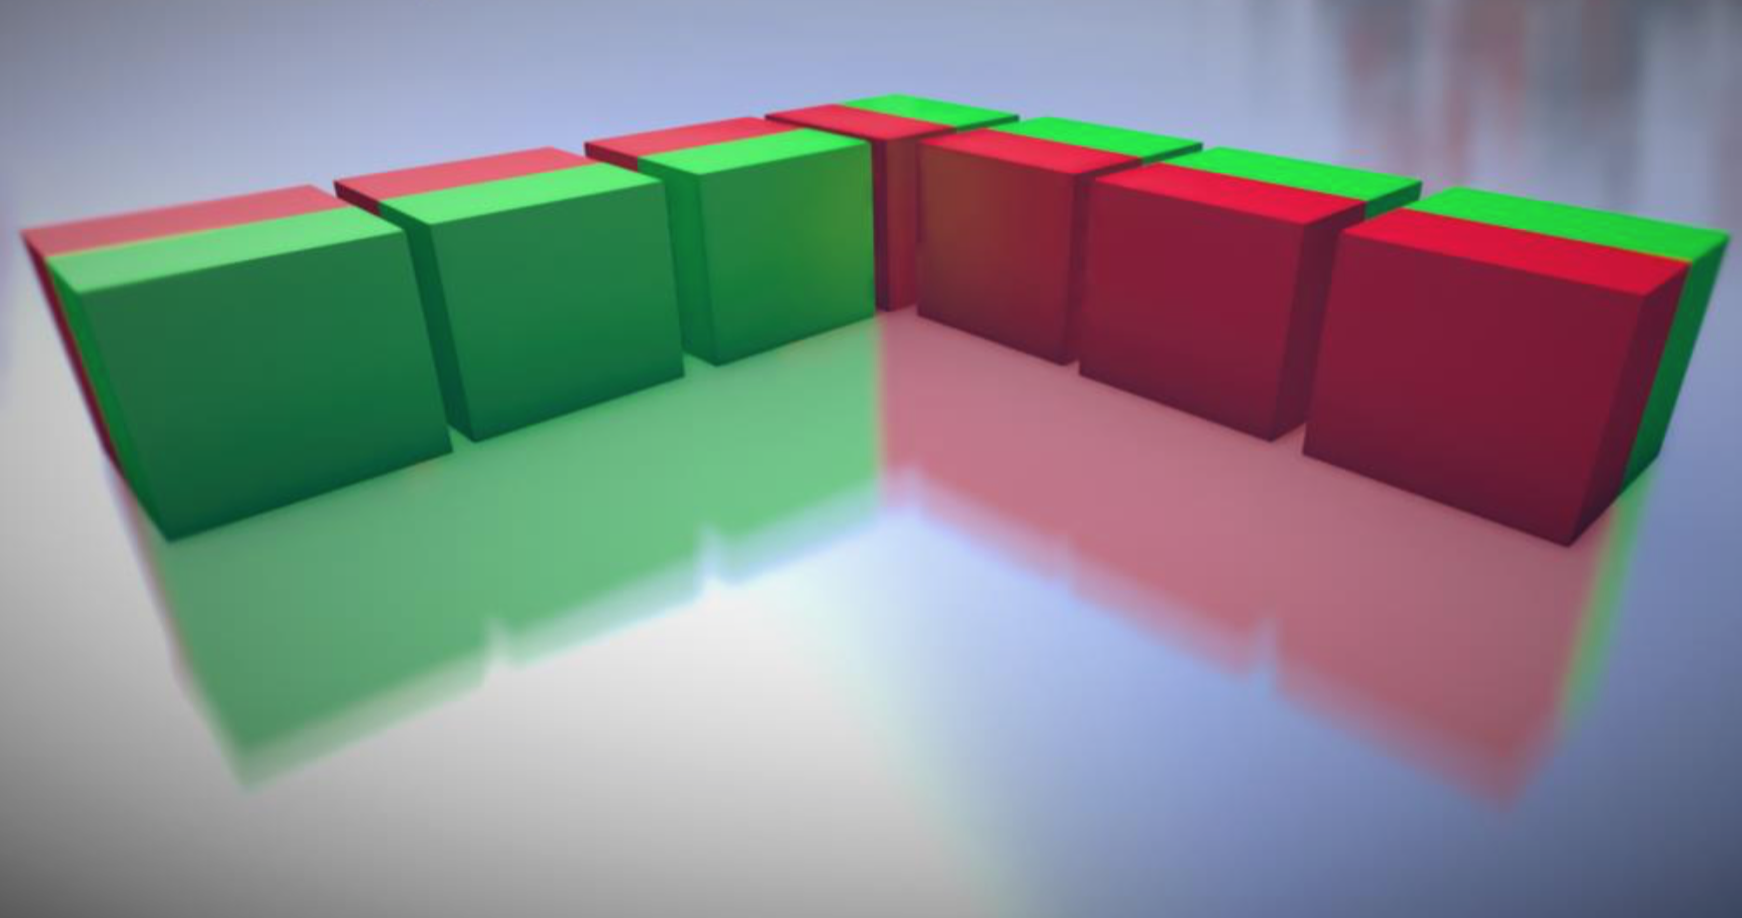
\includegraphics{graphics/vct/vct-11-2}
		\caption{Multicoloured boxes}
	\end{subfigure}
	\begin{subfigure}[b]{0.343\textwidth}
		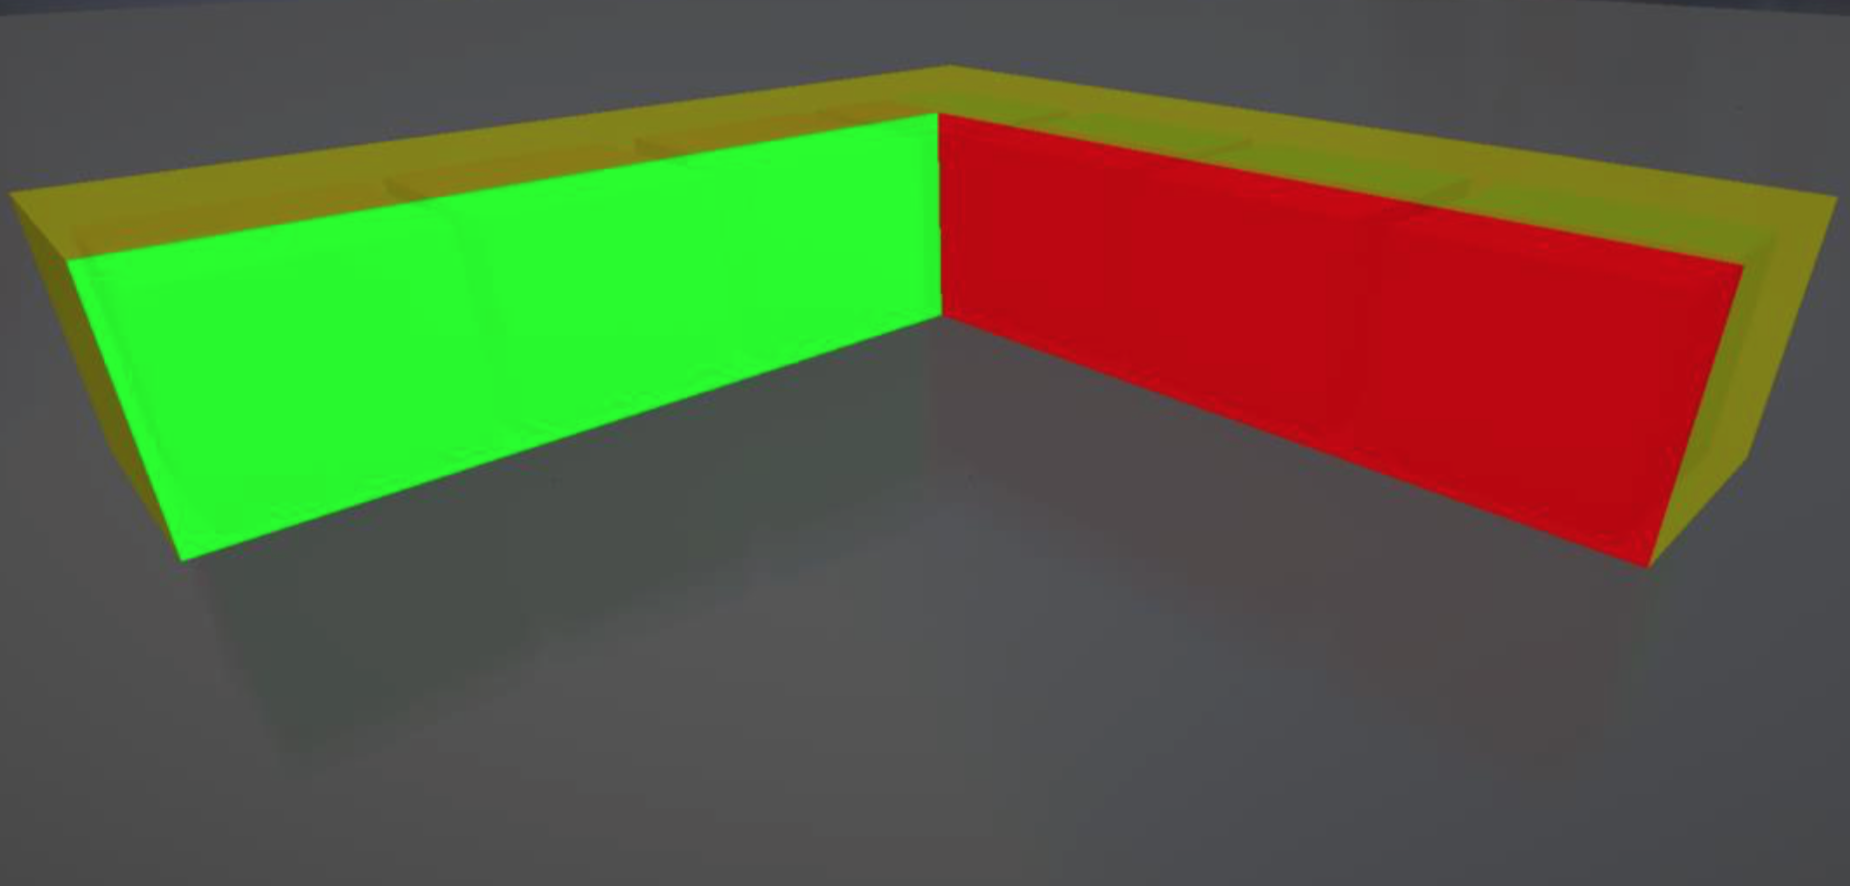
\includegraphics{graphics/vct/vct-11-3}
		\caption{Anisotropic voxels}
	\end{subfigure}
	\begin{subfigure}[b]{0.336\textwidth}
		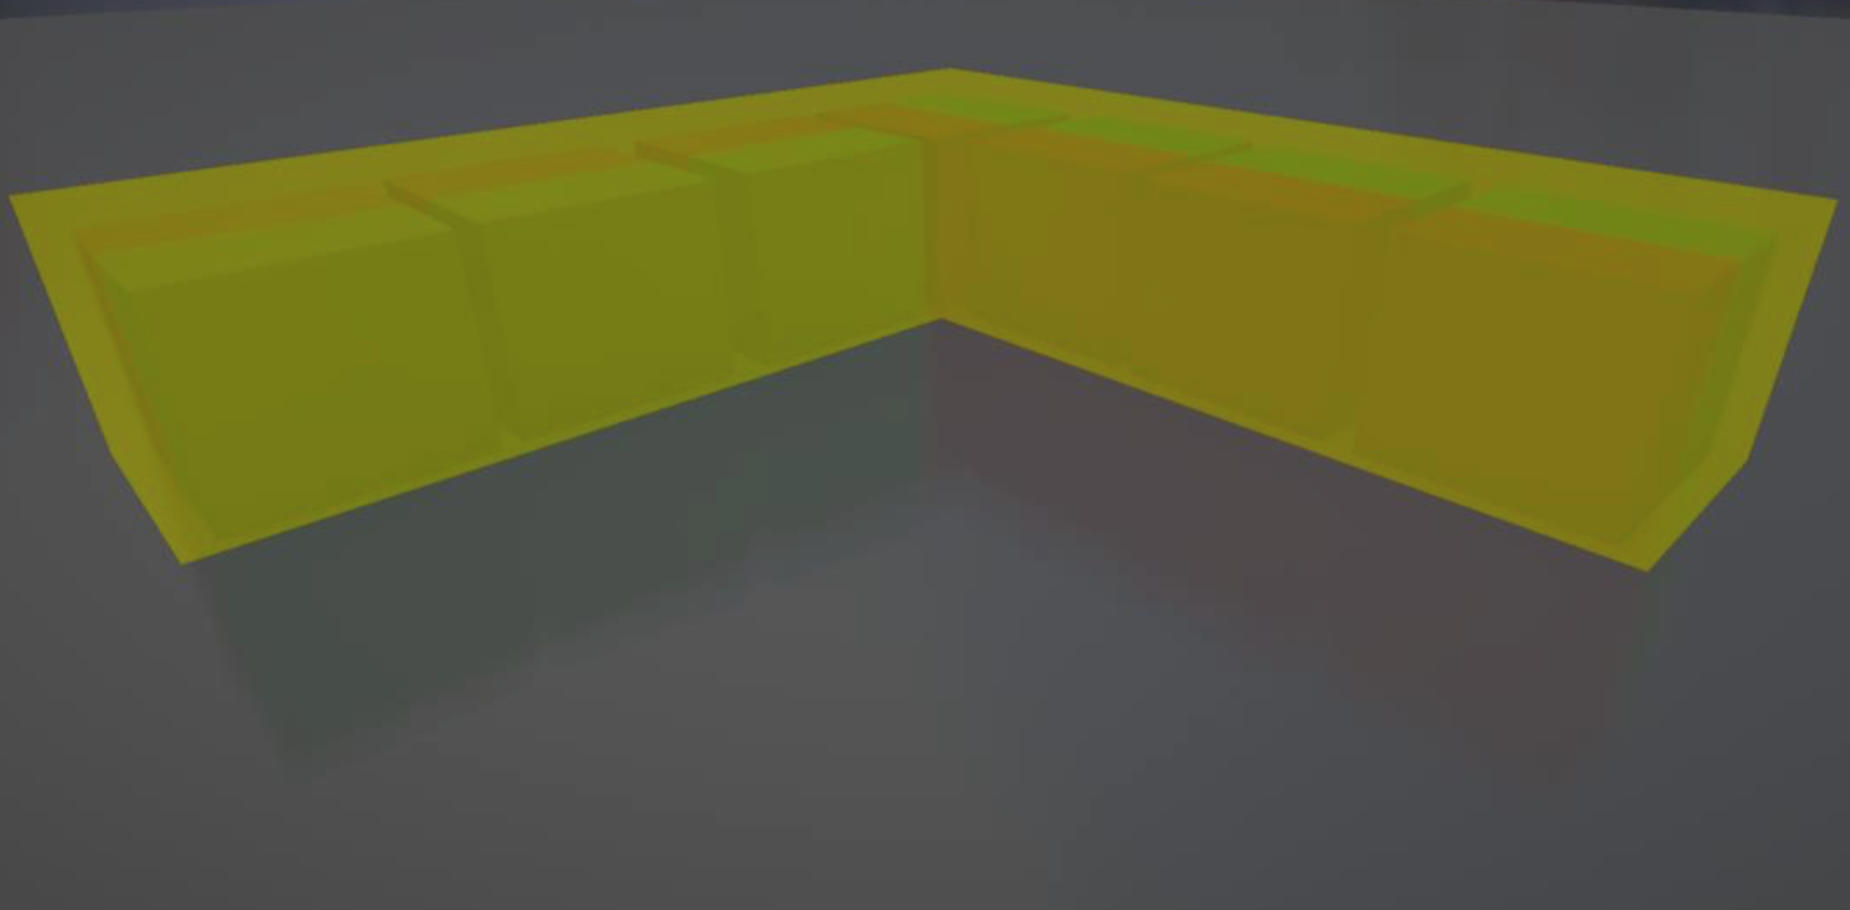
\includegraphics{graphics/vct/vct-11-4}
		\caption{Isotropic voxels}
	\end{subfigure}
	\caption{Some multicoloured boxes which each fit in a single voxel. The best we could do would be to somehow have pick one of the faces for the value of the albedo, or take an average of it, and do the same for our other attributes.}
\end{figure*}

Ideally, we would like to accurately encode the directional parameters $\mathbf{d}$ for both $\overline{T}(\mathbf{p},\mathbf{d},s,l)$ and $\overline{Q}(\mathbf{p},\mathbf{d},s,l)$ functions inside our MIP-map representation. This would allow a miapmapped voxel to be fully opaque when seen normally to the half set of opaque voxels, and half-transparent when seen tangentially to the set (see the right of figure \ref{f:vct-anisotropic-voxels}). In figure \ref{f:vct-anisotropic-voxels-1}, we would like the mipmapped voxel to be red when seen from the red side, green when seen from the green side, and a mix of the two when seen tangentially.

\begin{figure}\label{f:vct-anisotropic-voxels}
	\begin{subfigure}[b]{0.765\textwidth}
		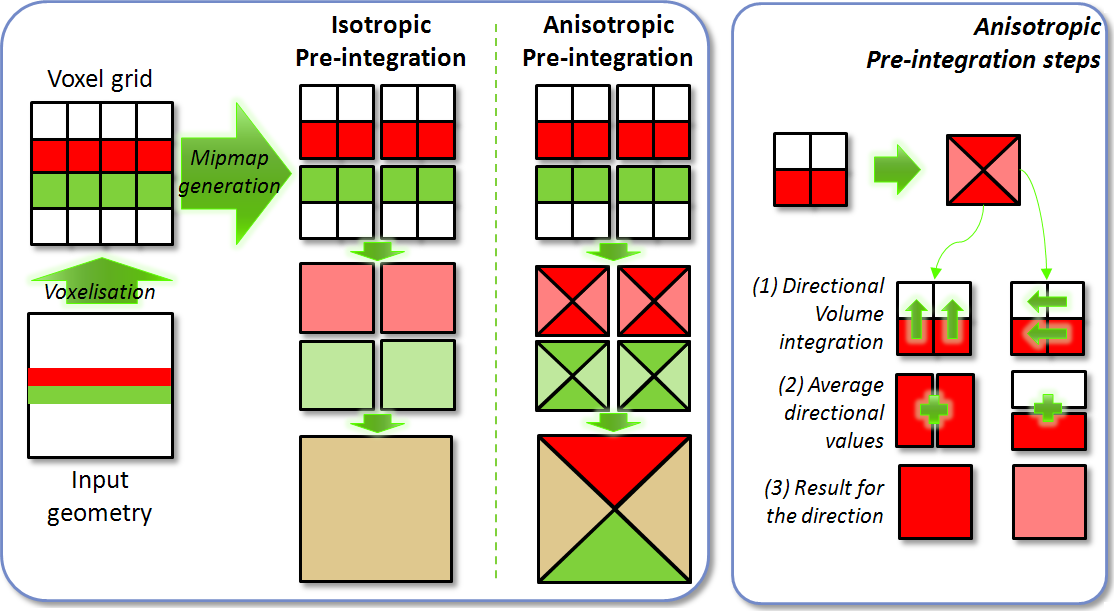
\includegraphics{graphics/vct/vct-10-1}
	\end{subfigure}
	\begin{subfigure}[b]{0.215\textwidth}
		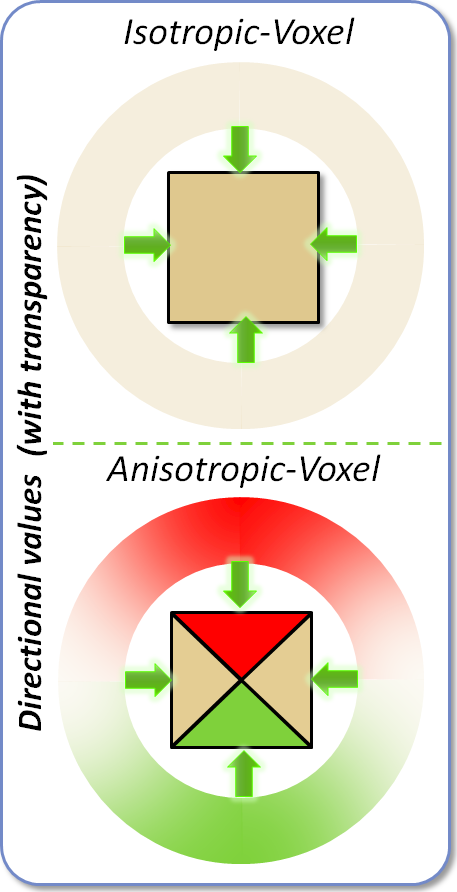
\includegraphics{graphics/vct/vct-10-2}
	\end{subfigure}
	\caption{The left blue box illustrates the voxel MIP- mapping process without (left) and with (right) anisotropic voxels and directional pre-integration. Directional integration steps are illustrated in the middle blue box. The right box shows the result of directional sampling of a voxel.}
\end{figure}

Storing values for a precise discretization of $\mathbf{d}$ would be very costly. To approach that goal, we propose an aniostropic voxel representation that is built during the MIP-mapping process, when building or updating the octree with irradiance values. Instead of a single channel of non-directional values, voxels store 6 channels of directional values, one per major direction. As illustrated in figure \ref{f:vct-anisotropic-voxels}, a directional value is computed by doing a step of volumetric integration in depth, and then averaging the 4 directional values to get the resulting value for one given direction. At render time, the voxel value is retrieved by linearly interpolating the values from the 3 directions closest to the direction the voxel is viewed. 

\begin{figure}\label{f:vct-anisotropic-voxels-2}
	\begin{subfigure}[b]{0.5\textwidth}
		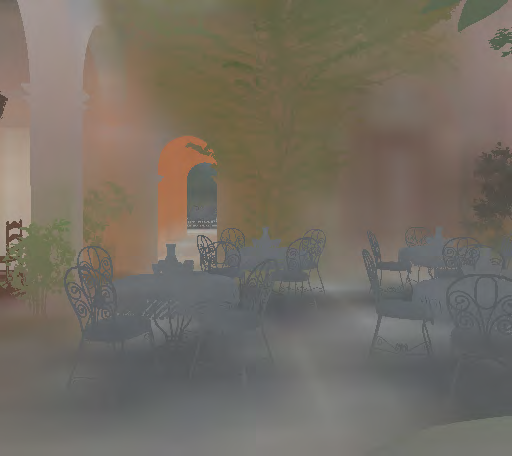
\includegraphics{graphics/vct/vct-12-1}
	\end{subfigure}
	\begin{subfigure}[b]{0.5\textwidth}
		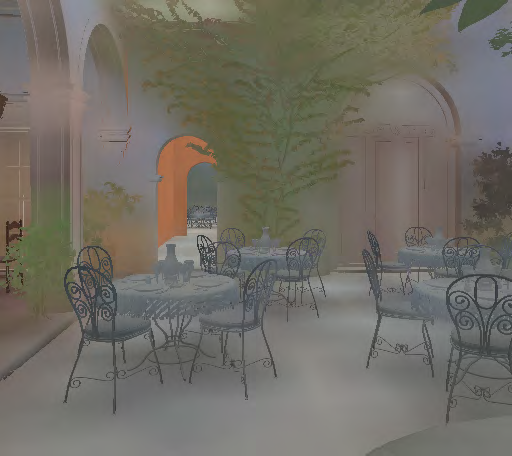
\includegraphics{graphics/vct/vct-12-2}
	\end{subfigure}
	\caption{Image comparison with direct voxel sampling on a proxy surface geometry from the octree between isotropic voxels (left) and anisotropic voxels (right). Observed voxel direction is given by the normal of the geometry.}
\end{figure}

This directional representation needs only to be used for voxels that are not at the full resolution and are not located in the last level of the octree. Thus, storing directional values for all the properties present in our structure only increases the memory consumption by $1.5\times$.

A comparison of image quality between isotropic and anisotropic pre-integrated voxel representations is presented in figure \ref{f:vct-anisotropic-voxels-2}. Voxels are sampled directly from a proxy surface geometry and voxel view direction is provided by the normal of the proxy geometry. One can observe that many more details can be captured and reproduced thanks to the isotropic voxel representation.





\section{Data Structure}
Our structure provides a compact storage of the dataset, allows a fast traversal for rendering operations and is easy to modify, allowing interactive updates. It provides a fast logarithmic complexity access to the entire dataset and all MIP-map resolutions. It is also designed to allow the storage of multiple scalar or vector material and shading parameters in order to allow the implementation of arbitrary shading models. 



\subsection{The Octree-based Voxel MIP-map Pyramid}
An adaptive space subdivision is essential to render large volumetric scenes and to adapt to memory limited environments. Such a hierarchical representation allows us to adapt the volume's internal resolution, to compact empty spaces, and to omit occluded parts according to the current point of view. This reduces enormously the memory consumption and avoids storing the entire information on the GPU, see figure \ref{f:vct-voxel-representation}.

\begin{marginfigure}
	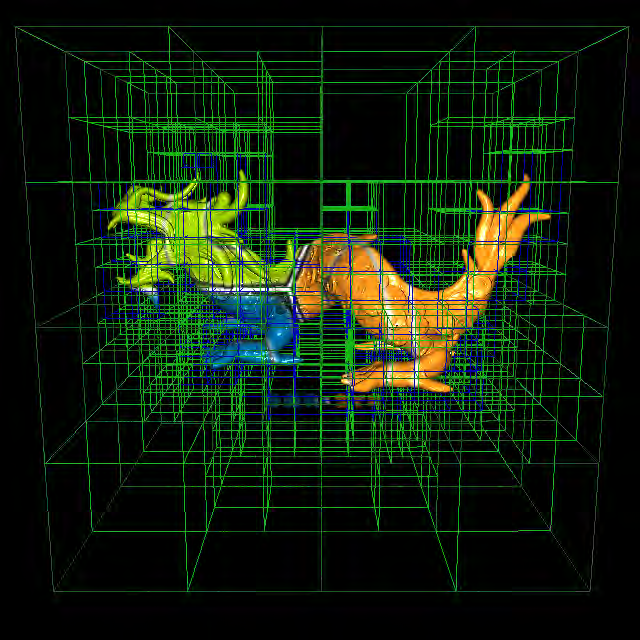
\includegraphics{graphics/vct/vct-13-1}
	\caption{Spatial partitioning of the octree structure. A voxelized version of the Stanford XYZRGB-Dragon model ($1024^{3}$ voxels) rendered at around 80F PS.}
	\label{f:vct-voxel-representation}
\end{marginfigure}



\subsection{GPU Representation}\label{sec:vct-gpu}
Our sparse voxel octree is a compact pointer-based structure, see figure \ref{f:vct-gpu-representation}. Octree nodes are stored in linear GPU memory and nodes are grouped into $2\times 2\times 2$ tiles. Further, each node contains a pointer to a small voxel volume, a \textit{brick}, stored in texture memory. This texture approximates the scene section represented by the node. 

Such a structure combines two major advantages: the octree leads to a compact storage (empty space skipping, occlusion culling, local refinement), whereas the bricks are implemented as small 3D textures and, thus, benefit from hardware-based interpolation and cache coherence. Another advantage is the constant size of the node and brick data types. Consequently, it is simple to store them densely in memory pools on the GPU. This facilitates the update mechanisms which are crucial to ensure the presence of the data needed to produce the output image.

\begin{figure}\label{f:vct-gpu-representation}
\begin{center}
	\begin{subfigure}[b]{0.4\textwidth}
		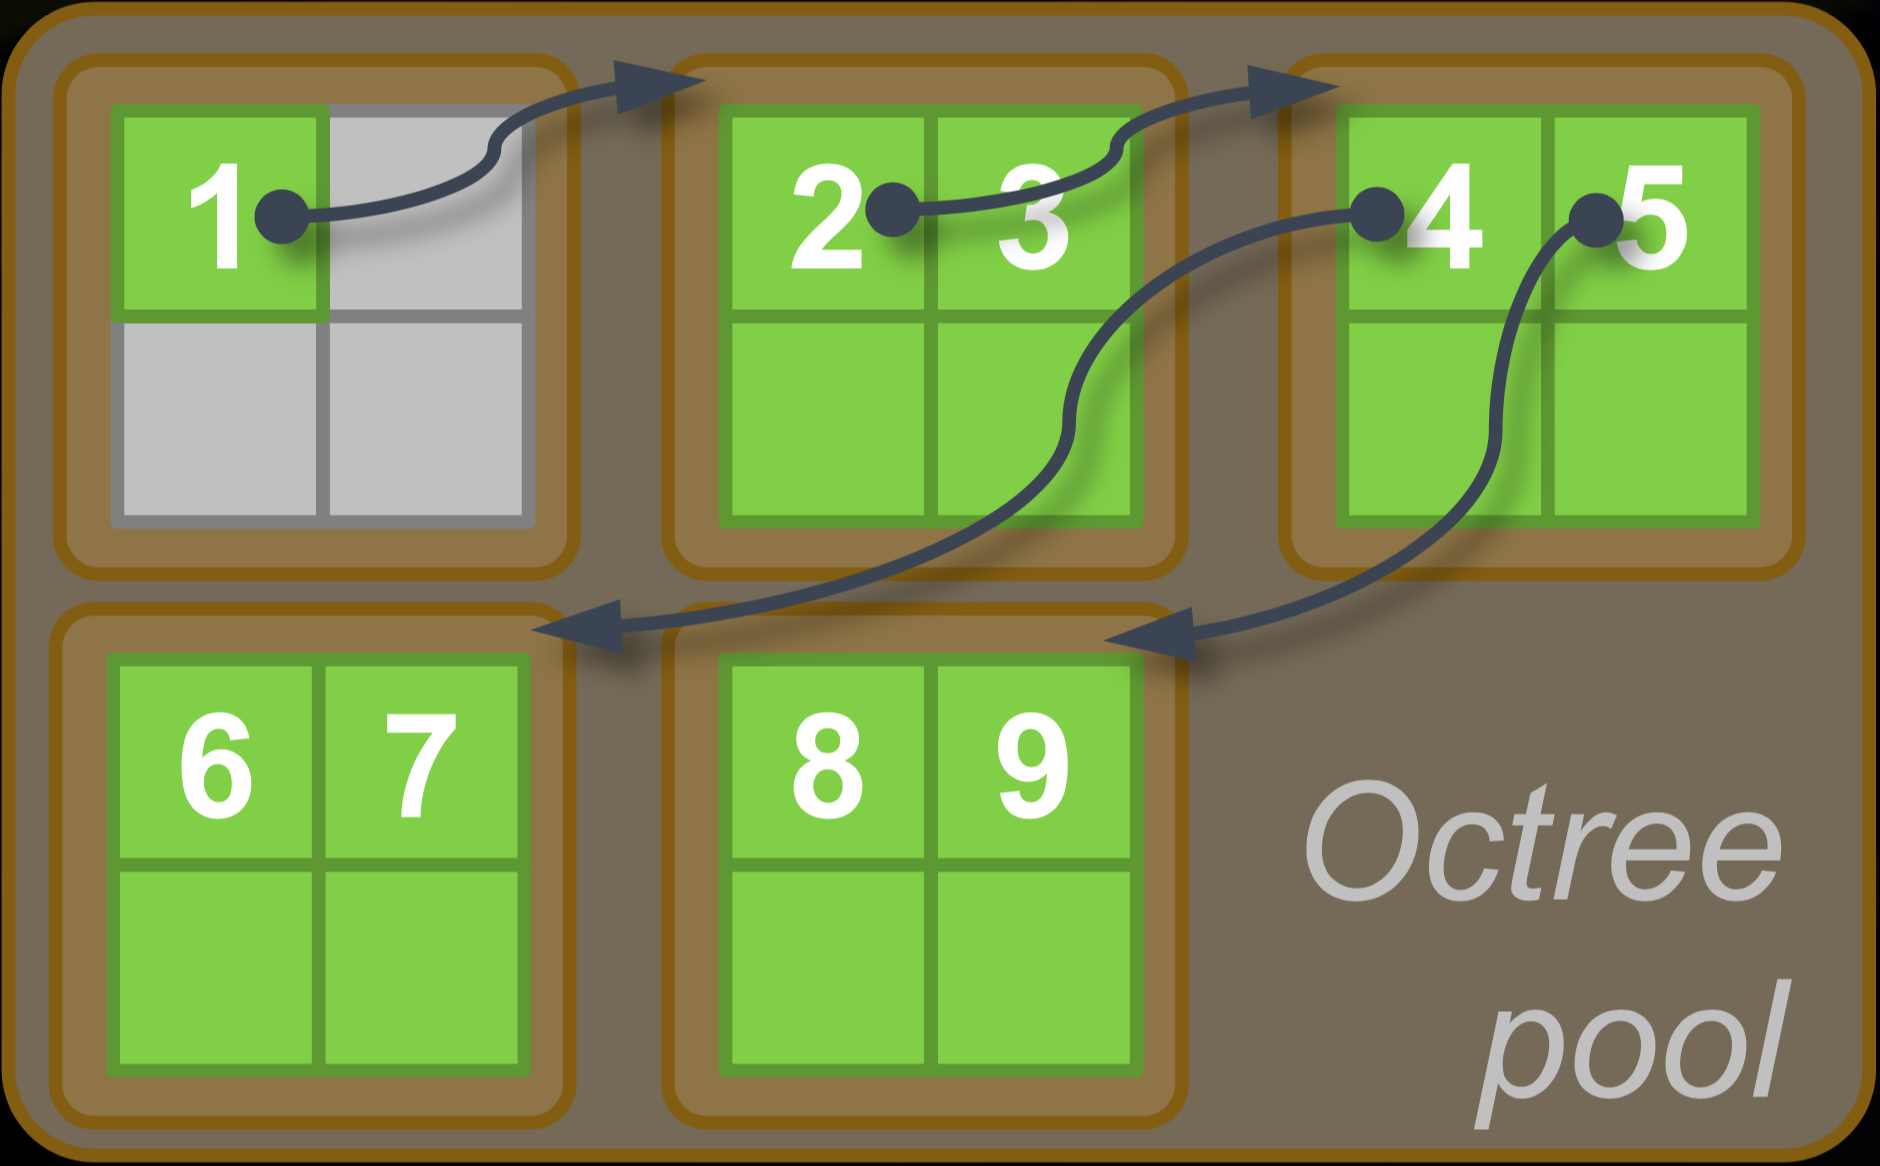
\includegraphics{graphics/vct/vct-13-8}
	\end{subfigure}
	\begin{subfigure}[b]{0.4\textwidth}
		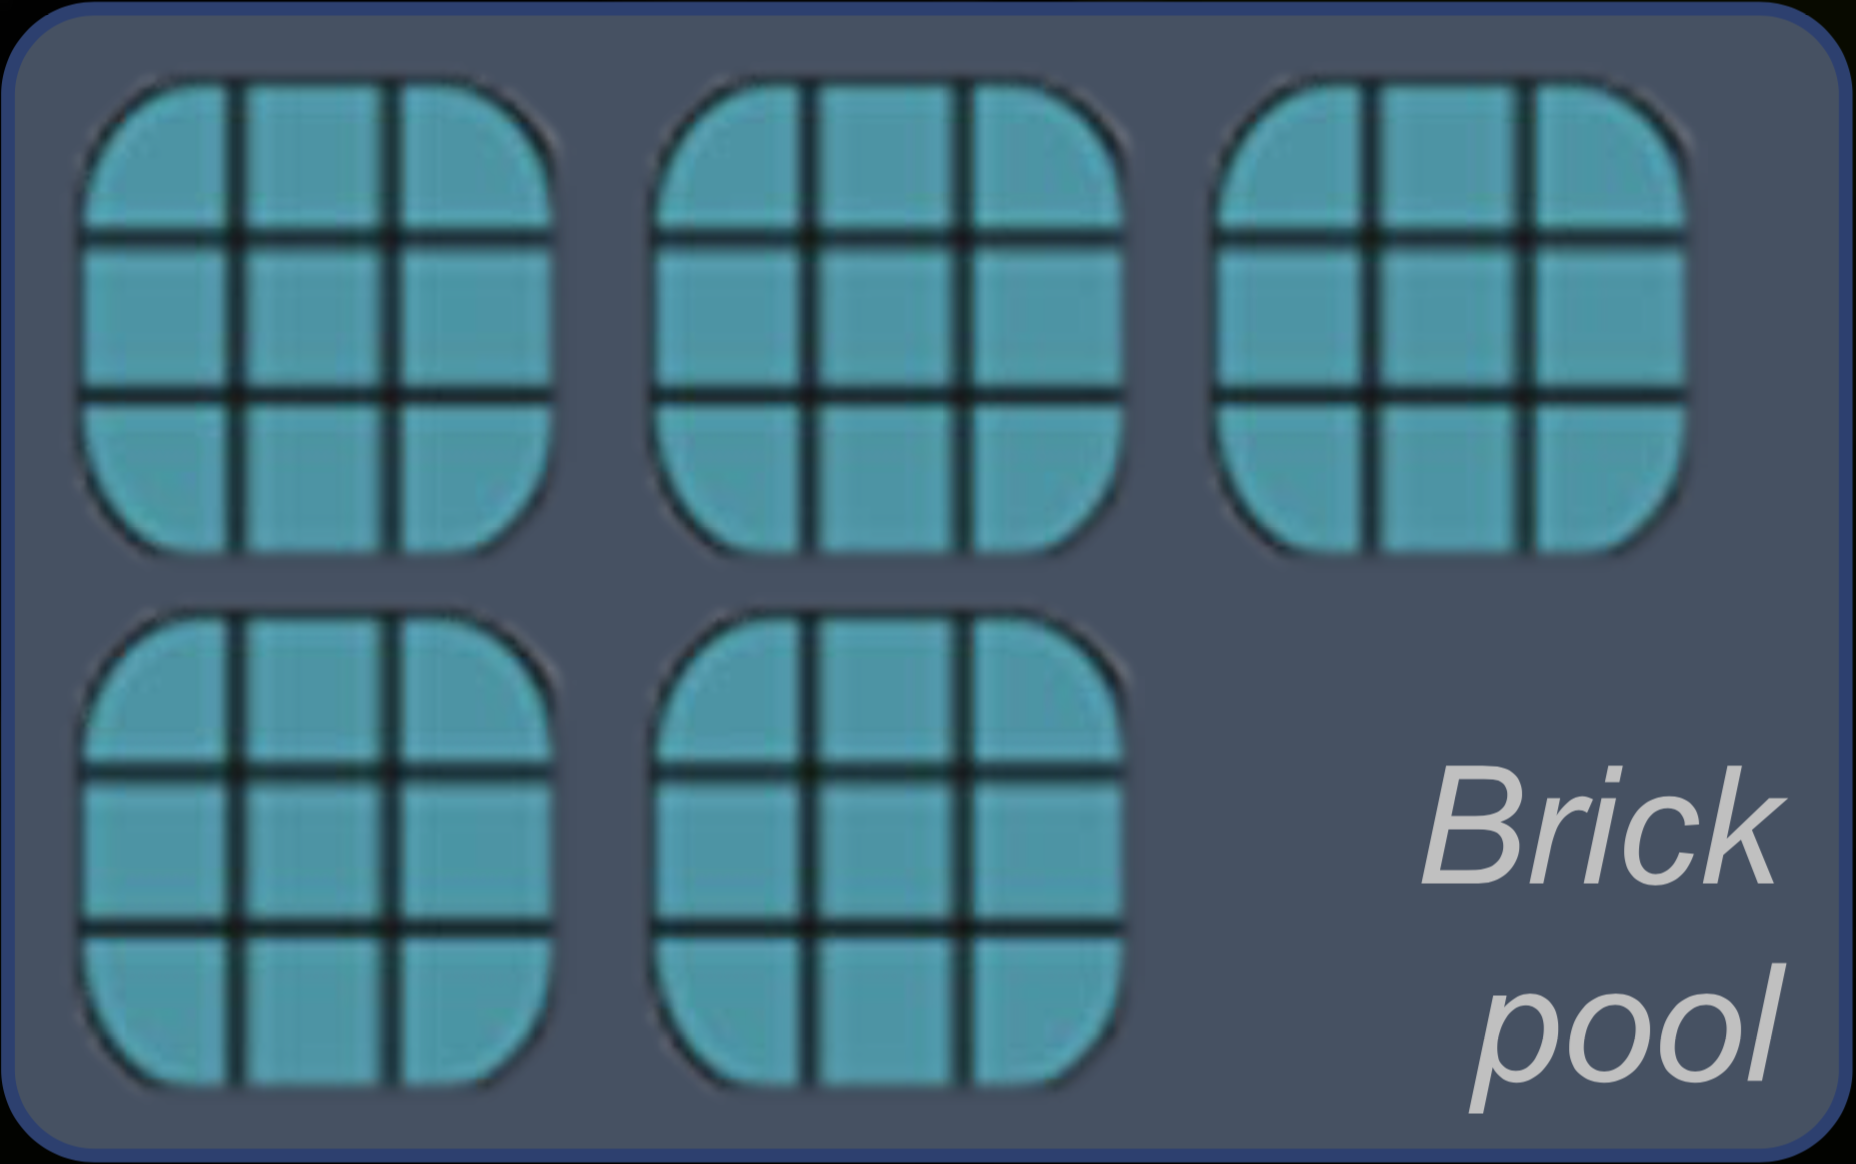
\includegraphics{graphics/vct/vct-13-9}
	\end{subfigure}
\end{center}
	\caption{Our sparse voxel octree data structure. This structure stores a whole voxel scene or object filtered at multiple resolutions. Bricks are referenced by octree nodes providing a sparse MipMap pyramid of the voxels.}
\end{figure}




\subsubsection{The Bricks}
The 3D bricks linked by the nodes at each level of the octree are used to provide a fast and interpolated access to the actual voxel data. They are stored inside texture memory allowing them to benefit from the support of hardware accelerated interpolation and 3D-local cache. Each brick voxel can store multiple channels of values used for rendering, usually at least a color, an opacity and a normal distribution (for shading). 

In order to ensure a correct trilinear interpolation by the hardware at brick boundaries, some voxels must be replicated between adjacent bricks. But such brick representation proposed by \cite[-20mm]{a:InteractiveIndirectIlluminationUsingVoxelConeTracing} is not optimal in case of small bricks, due to the need of a one voxel border duplicating neighboring voxels. This border becomes very expensive in terms of storage when small bricks are used.

\begin{marginfigure}
	\begin{center}
		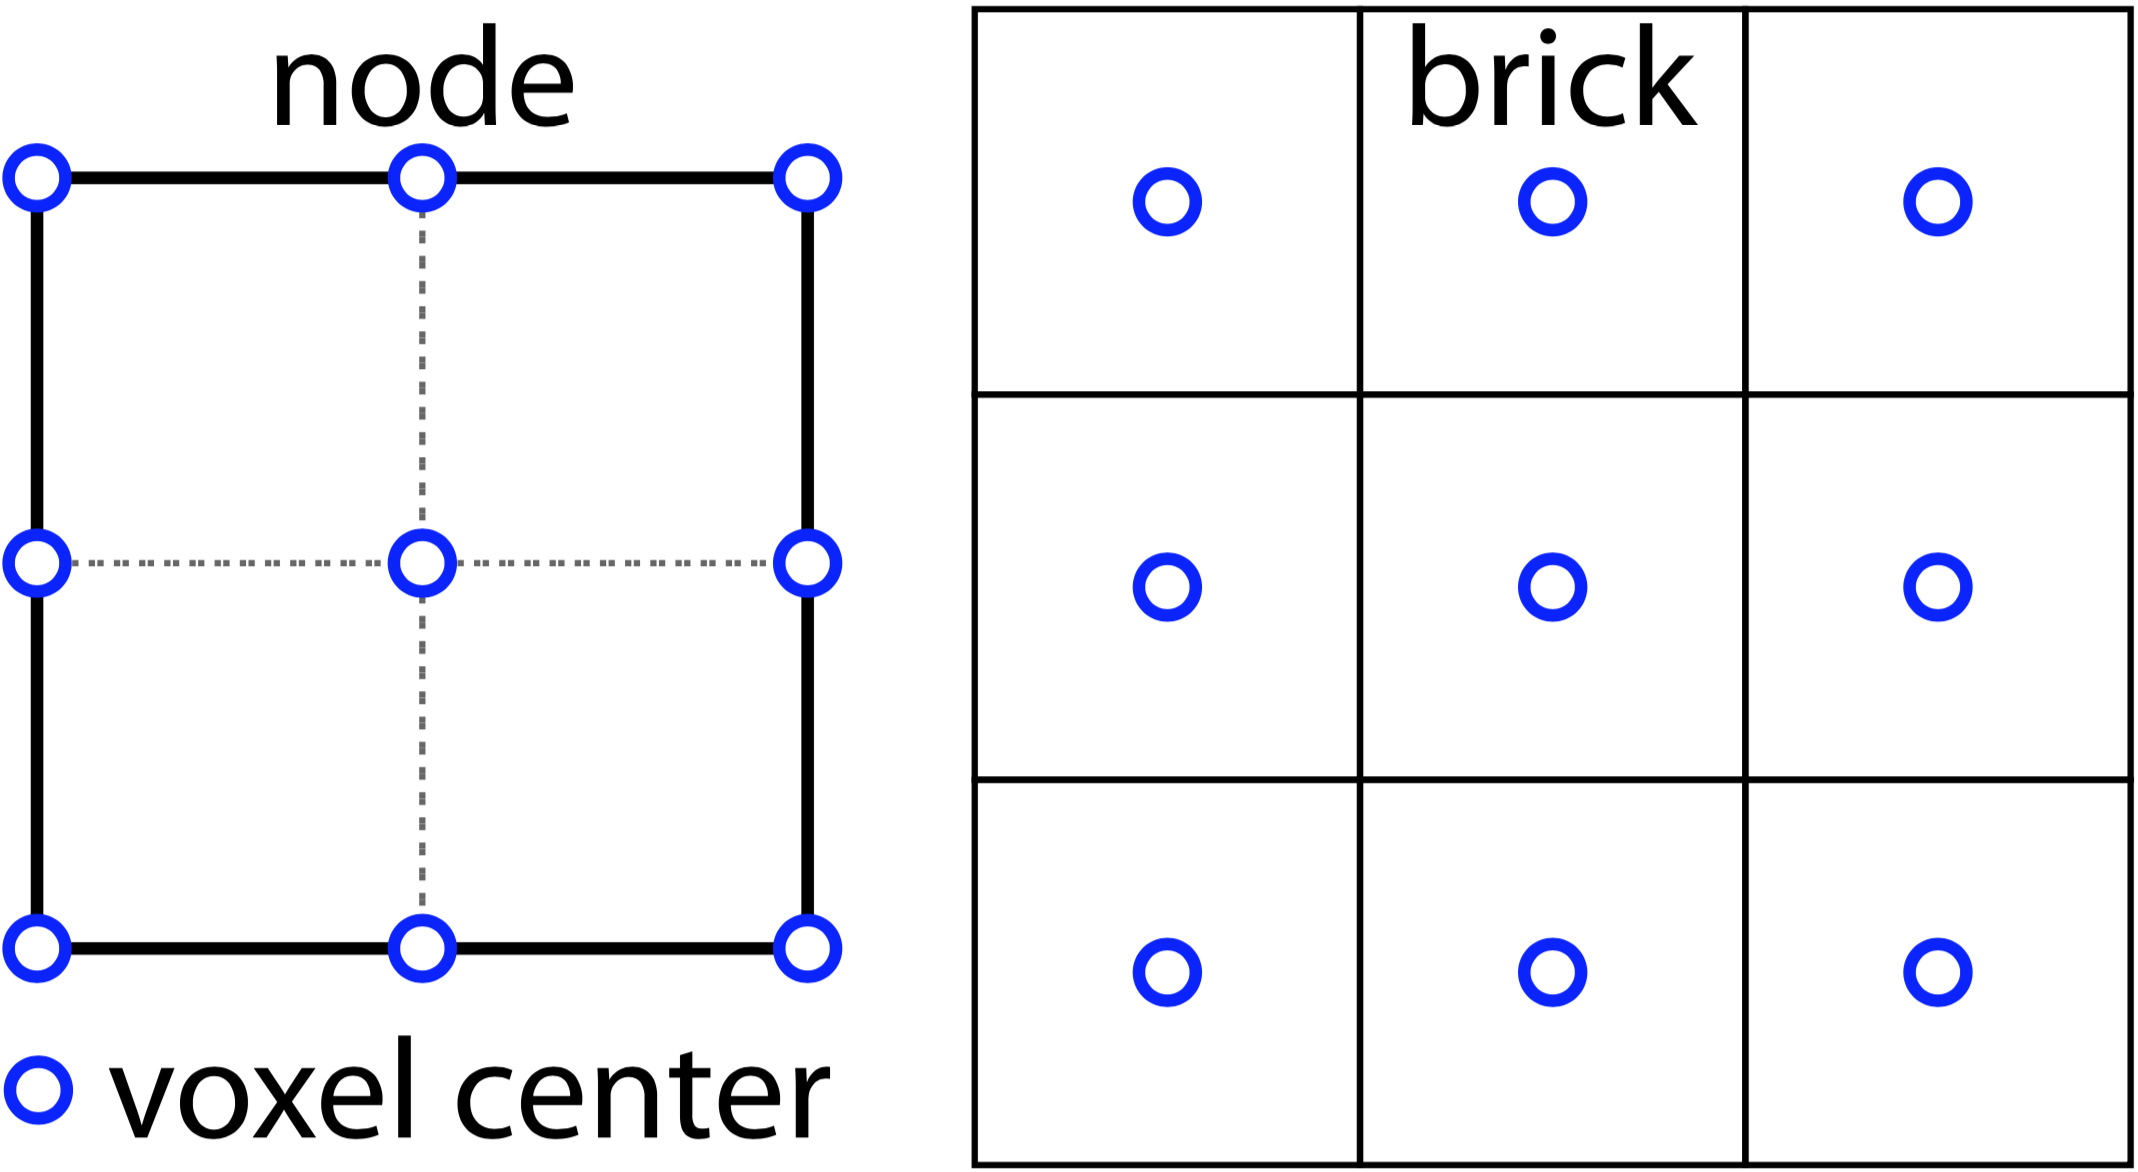
\includegraphics{graphics/vct/vct-13-11}
	\end{center}
	\caption{The representation of a brick.}
\end{marginfigure}

To solve this problem, we propose to use $3\times 3\times 3$ voxel bricks, but assume that the voxel centers are located at the node corners instead of the node centers, see the left of figure \ref{f:vct-bricks}. This ensure that interpolated values can always be computed inside a brick covering a set of $2\times 2\times 2$ nodes. Redundancy is not eliminated, but we use less than half the amount of memory compared to adding a boundary, for the same sampling precision. 

This memory reduction allows us to add neighbor pointers to the structure which enable us to quickly visit spatially neighboring nodes and the parent. We will see that these links are particularly important to efficiently distribute the direct illumination over all levels of the tree.




\subsection{Octree Construction and Update}
Our sparse hierarchical voxel structure will replace the actual scene in our light transport computations. The voxel data representation allows interpolation and filtering computations to be simple.

Both semi-static and fully dynamic objects are stored in the same octree structure for an easy traversal and unified filtering. A time-stamp mechanism is used to differentiate both types, in order to prevent semi-static parts of the scene to be destructed in each frame. Our structure construction algorithm performs in two steps: octree building and dynamic update.



\subsubsection{Octree Building}
We first create the octree structure itself by using the GPU rasterization pipeline. We rasterize the mesh three times, along the three main axis of the scene, with a viewport resolution corresponding to the resolution of the maximum level of subdivision of the  octree (typically $512\times 512$ pixels for a $512^{3}$ octree). By disabling the depth test to prevent early culling, we generate at least one fragment shader thread for each potentially-existing leaf node in the tree. Each thread traverse the octree from top-to-bottom and directly subdivide it when needed. Once the correct leaf node is found the surface attributes (typically texture color, normal and material) are written. 

Whenever a node needs to be subdivided, a set of $2\times 2\times 2$ sub-nodes are "allocated" inside a global shared \textit{node buffer} which is per-allocated in video memory. The address of this set of new sub-nodes is written to the "child" pointer of the subdivided node and the thread continue its descent down to the leaf. These allocations are made using the atomic increment of a global shared count, which indicates the next available page of nodes in the shared node buffer. Since, in a massively parallel environment, multiple threads can request the subdivision of the same node at the same time an incoherent structure could result. Such conflicts are prevented by a per-node mutex that ensures that the subdivision is only performed by the first thread. Unfortunately, it is not possible to put the other threads asleep while waiting for the first thread to finish the subdivision.

In order to avoid an active waiting loop would be too expensive, we implemented a \textit{global thread list} where interrupted threads put themselves for a deferred execution. At the end of the rasterization pass, deferred threads are re-run (in a vertex shader) and their values written in the tree. Such deferred passes can possibly generate new deferred threads and are re-executed as long as the global thread list is not empty. Values in the leaves are written directly inside the brick associated to the nodes, and bricks are allocated similarly to the nodes inside a \textit{shared brick buffer}. 




\subsubsection{Dynamic Update}
Dynamic update of the octree structure for animated objects is done with the same rasterization-based building algorithm we just described. Animated objects are rasterized every frame, the only difference is that new voxels generated by these objects cannot overwrite existing static parts of the structure. To prevent overwriting static octree nodes and bricks, and allow for a fast clearing every frame, these elements are stored at the end of the buffers.





\section{Rendering}
So now we know what cone tracing is, and how we're roughly going to store our scene, let's look at how to use that to get some global illumination. This approach is based on a three-step algorithm as detailed in figure \ref{f:vct-steps}:

\begin{figure}\label{f:vct-steps}
	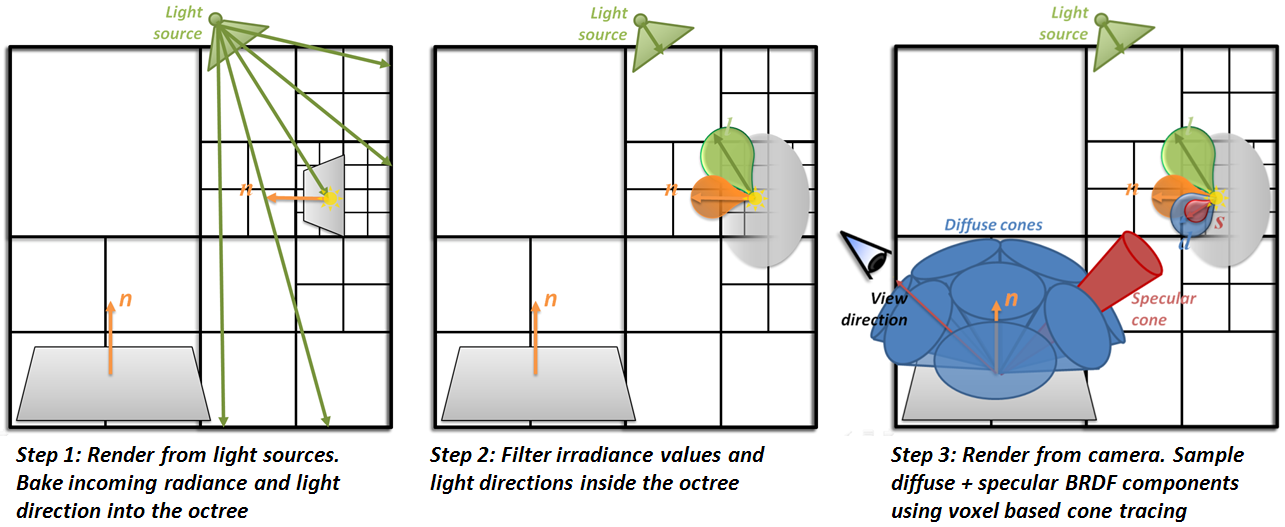
\includegraphics{graphics/vct/vct-3}
	\caption{Illustration of the three steps of our real-time indirect lighting algorithm.}
\end{figure}

\begin{itemize}
	\item First, we inject incoming radiance (energy and direction) from dynamic light sources into the leaves of the sparse voxel octree hierarchy. This is done by rasterizing the scene from all light sources and splatting a photon for each visible surface fragment.
	\item Second, we filter the incoming radiance values into the higher levels of the octree (mipmap). We rely on a compact Gaussian-Lobes representation to store the filtered distribution of incoming light directions, which is done efficiently in parallel by relying on a screen-space quad-tree analysis.
	\item Finally, we render the scene from the camera. For each visible surface fragment, we combine the direct and indirect illumination. We employ an approximate cone tracing to perform a final gathering, sending out a few cones over the hemisphere to collect illumination distributed in the octree.
\end{itemize}




\subsection{Approximate Voxel Cone Tracing}
Global illumination generally requires many sampling rays to be test against scene, which is expensive. These rays are spatially and directionally coherent which is a property that many approaches such as packet ray-tracing use\cite[-10mm]{a:InteractiveRenderingwithCoherentRayTracing} (see section \ref{sec:coherent-ray-tracing}). Similarly, in order for us to exploit this coherence, we introduce a voxel cone tracing method that was inspired by filtering for anti-aliasing\cite{a:RayTracingwithCones}. 

While the original cone tracing technique is complex and often expensive, we can use our filtered voxel structure to approximate the result for all rays in the same bundle in parallel. The idea is to step along the cone axis and perform lookups in our hierarchical representation at the level corresponding to the cone radius (see figure \ref{f:vct-approximate-voxel-cone-tracing}). During this step, we use quadrilinear interpolation to ensure a smooth variation that does not exhibit aliasing. Because of the way we pre-filtered the voxel data, this approximation produces visual plausible results although it might differ from true tracing. 

\begin{figure}\label{f:vct-approximate-voxel-cone-tracing}
	\begin{center}
		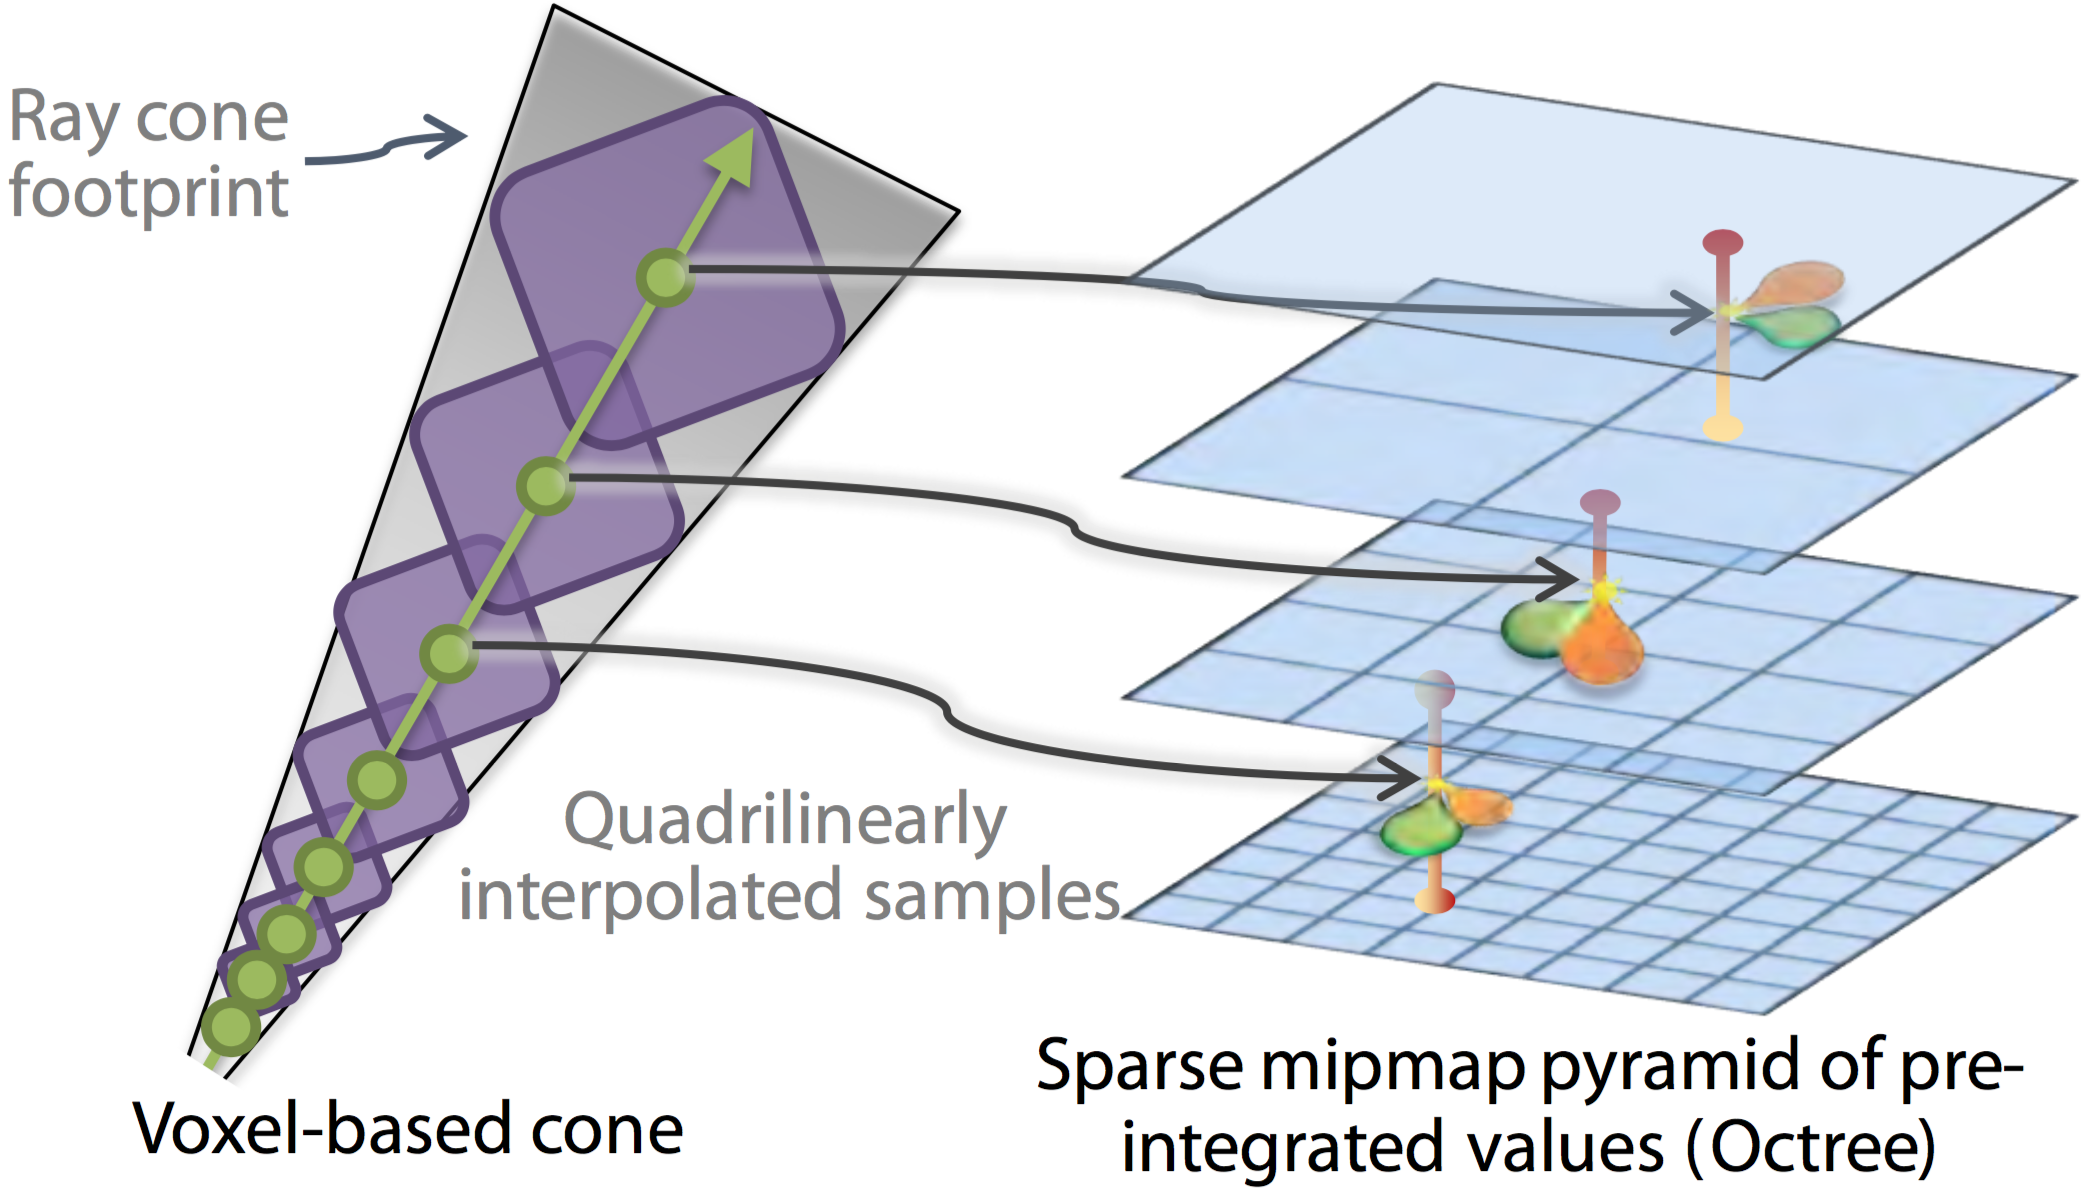
\includegraphics[width=0.7\textwidth]{graphics/vct/vct-7-4}
	\end{center}
	\caption{Voxel-based cone tracing using pre-filtered geometry and lighting information from a sparse MIP-map pyramid (stored in a voxel octree structure).}
\end{figure} 

While stepping along the cone, we use the classical emission-absorption optical model to accumulate the values along the cone. We keep track of occlusion $\alpha$ and , potentially, a color value $c$ representing the reflected light towards the cone origin. In each step, we retrieve the appropriately filtered scene information and the occlusion value $\alpha_2$ from the octree to compute a new outgoing radiance $c_2$. We then update the values using the classical volumetric front-to-back accumulation: 

\begin{equation*}
	\begin{aligned}
		c:=&\alpha c+(1-\alpha)\alpha_2c_2\\
		\alpha=&\alpha+(1-\alpha)\alpha_2
	\end{aligned}
\end{equation*}

Also, to ensure good integration quality, even for large cones, the distance $d^{'}$ between successive sample locations along a ray does not coincide with the current voxel size $d$. To account for the smaller step size, we use the correction $\alpha^{/}_s=1-(1-\alpha_s)^{\frac{d^{'}}{d}}$. 





\subsection{Ambient Occlusion}
To illustrate the use of our approximate cone tracing and to facilitate the understanding of our indirect illumination algorithm, we will first present a simpler case: an ambient occlusion estimation (AO), which can be seen as an accessibility value. The ambient occlusion $A(p)$ at a surface point $p$ is defined as the visibility integral over the hemisphere $\Omega$ with respect to the projected solid angle. Precisely:

\begin{equation*}
	A(p)=\frac{1}{\pi}\int_\Omega V(p,\omega)cos\omega d\omega
\end{equation*}

where $V(p,\omega)$ is the visibility function that is zero if the ray originating at $s$ in direction $\omega$ intersects the scene, else it is one. For practical uses (typically, indoor scenes which have no open sky) the visibility is limited to a distance since the environment walls pay the role of ambient diffusors. Hence, we weight occlusion $\alpha$ by a function $f(r)$ which decays with the distance (in this implementation we use $\frac{1}{1+\lambda r}$). The modified occlusion is:

\begin{equation*}
	\alpha_f(p+r\omega):=f(r)\alpha(p+r\vec{\omega})
\end{equation*}

To compute the integral $A(p)$ efficiently, we observe that the hemisphere can be partitioned into a sum of integrals: 

\begin{equation*}
\begin{aligned}
	A(p)=&\frac{1}{N}\sum^{N}_{i=1}Vc(p,\Omega_i)\text{, where }\\
	Vc(p,\Omega_i)=&\int_{\Omega}V_{p,\theta}cos\theta d\theta
\end{aligned}
\end{equation*}

\begin{marginfigure}
	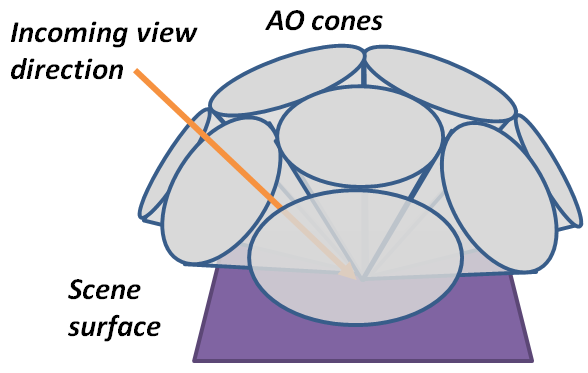
\includegraphics{graphics/vct/vct-14-1}
	\caption{Ambient Occlusion with a small set of voxel cones.}
	\label{f:vct-ao}
\end{marginfigure}

For a regular partition, each $Vc(p,\Omega_i)$ resembles a cone. If  we factor the cosine out of the $Vc$ integral (the approximation is coarse mainly for large or grazing cones), we can approximate their contribution with our voxel-based cone tracing, as illustrated in figure \ref{f:vct-ao}. The weighted visibility integral $V(p,\omega)$ is obtained by accumulating the occlusion information only, accounting for the weight $f(r)$. Summing up contributions of all cones results in our approximation of the AO term.




\subsection{Indirect Illumination}
To compute indirect illumination in the presence of a point light is more involved than AO. We use on a two-step approach. First, we capture the incoming radiance from a light source in the leaves of our scene representation. Storing incoming radiance, not outgoing will allow us to simulate glossy surfaces. We filter and distribute the incoming radiance over all levels of our octree. Finally, we perform approximate cone tracing to simulate the light transport. Writing the incoming radiance in the octree structure is complex, therefore we will, for the moment, assume that it is already present in our octree structure, before detailing this process.

\begin{figure}\label{f:vct-indirect}
\begin{center}
	\begin{subfigure}[b]{0.48\textwidth}
		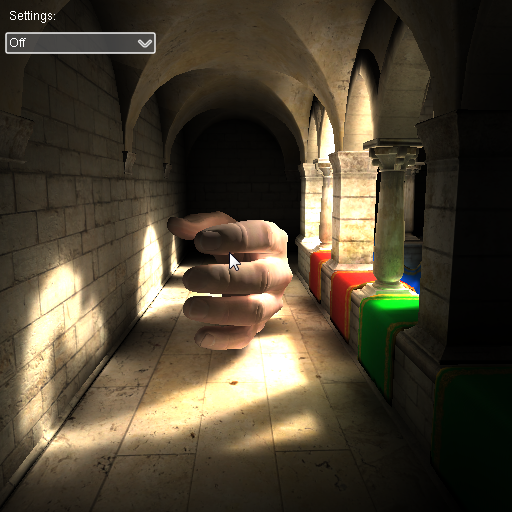
\includegraphics{graphics/vct/vct-14-2}
	\end{subfigure}
	\begin{subfigure}[b]{0.48\textwidth}
		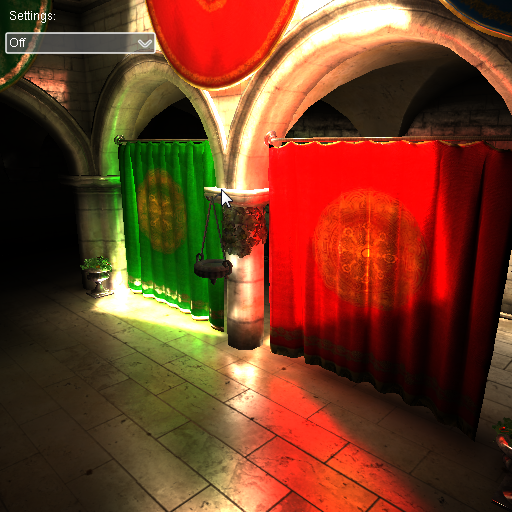
\includegraphics{graphics/vct/vct-14-3}
	\end{subfigure}
\end{center}
	\caption{Left: Indirect diffuse lighting with animated object. Right: Glossy reflections and color bleeding.}
\end{figure}




\subsubsection{Two-bounce Indirect Illumination}
Our solution works for low-energy/low-frequency and high-energy/high-frequency components of arbitrary material BRDFs, although we will focus our description on a Phong BRDF. The algorithm is similar to the one described in the previous section for AO. We use deferred shading to determine for which surface points we need to compute the indirect illumination. At each such location, we perform a final gathering by sending out several cones to query the illumination that is distributed in the octree. Typically, for a Phone material, the right of figure \ref{f:vct-ao}, a few large cones (typically 5) estimate the diffuse energy coming from the scene, while a tight cone in the reflected direction with respect to the viewpoint captures the specular component. The aperture of the specular cone is derived from the specular exponent of the material, allowing us to compute glossy reflections.




\subsubsection{Capturing Direct Illumination}
Now we discuss how to store incoming radiance. Inspired by Reflective Shadow Maps\cite{a:ReflectiveShadowMaps}, we render the scene from the light's view using standard rasterization to output a world position.  Basically, each pixel represents a photon that we want to bounce in this scene. We call this map the \textit{light-view map}. In the following, we want to store these photons in the octree representation. Precisely, we want to store them as a direction distribution and an energy proportional to the subtended solid angle of the pixel as see from the light.

To splat the photons, we basically use a fragment shader with one thread per light-view-map pixel. Because the light-view map's resolution is usually higher than the lowest level of the voxel grid, we can assume that we can spat photons directly into leaf nodes of our octree without introducing gaps. Furthermore, photons can always be placed at the finest level of our voxel structure because they are stored at the surface, and we only collapsed empty voxels to produce our sparse representation. Because several photons might end up in the same voxel, we need to reply on an atomic add.

Although the process sounds simple, it is more involved than one might think and there are two hurdles to overcome. The first problem is that atomic add operations are currently only available for integer textures. We can easily address this issue by using a 16bit normalized texture format, that is denormalized when accessing the value later. The second difficulty is that voxels are repeated for adjacent bricks. We mentioned in section \ref{sec:vct-gpu} that this redundancy is necessary for fast hardware-supported filtering. While thread collisions are rare for the initial splat, we found that copying the photon directly to all required locations in adjacent bricks leads to many collisions that affect performance significantly. This parallel random scattering, further, results in bandwidth issues. A more efficient transfer scheme is needed.




\subsubsection{Value Transfer to Neighboring Bricks}
In order to simplify the explanation, let's consider that our octree is complete, so that we can then launch one thread per leaf node.

\begin{figure}\label{f:vct-value-transfer}
	\begin{center}
		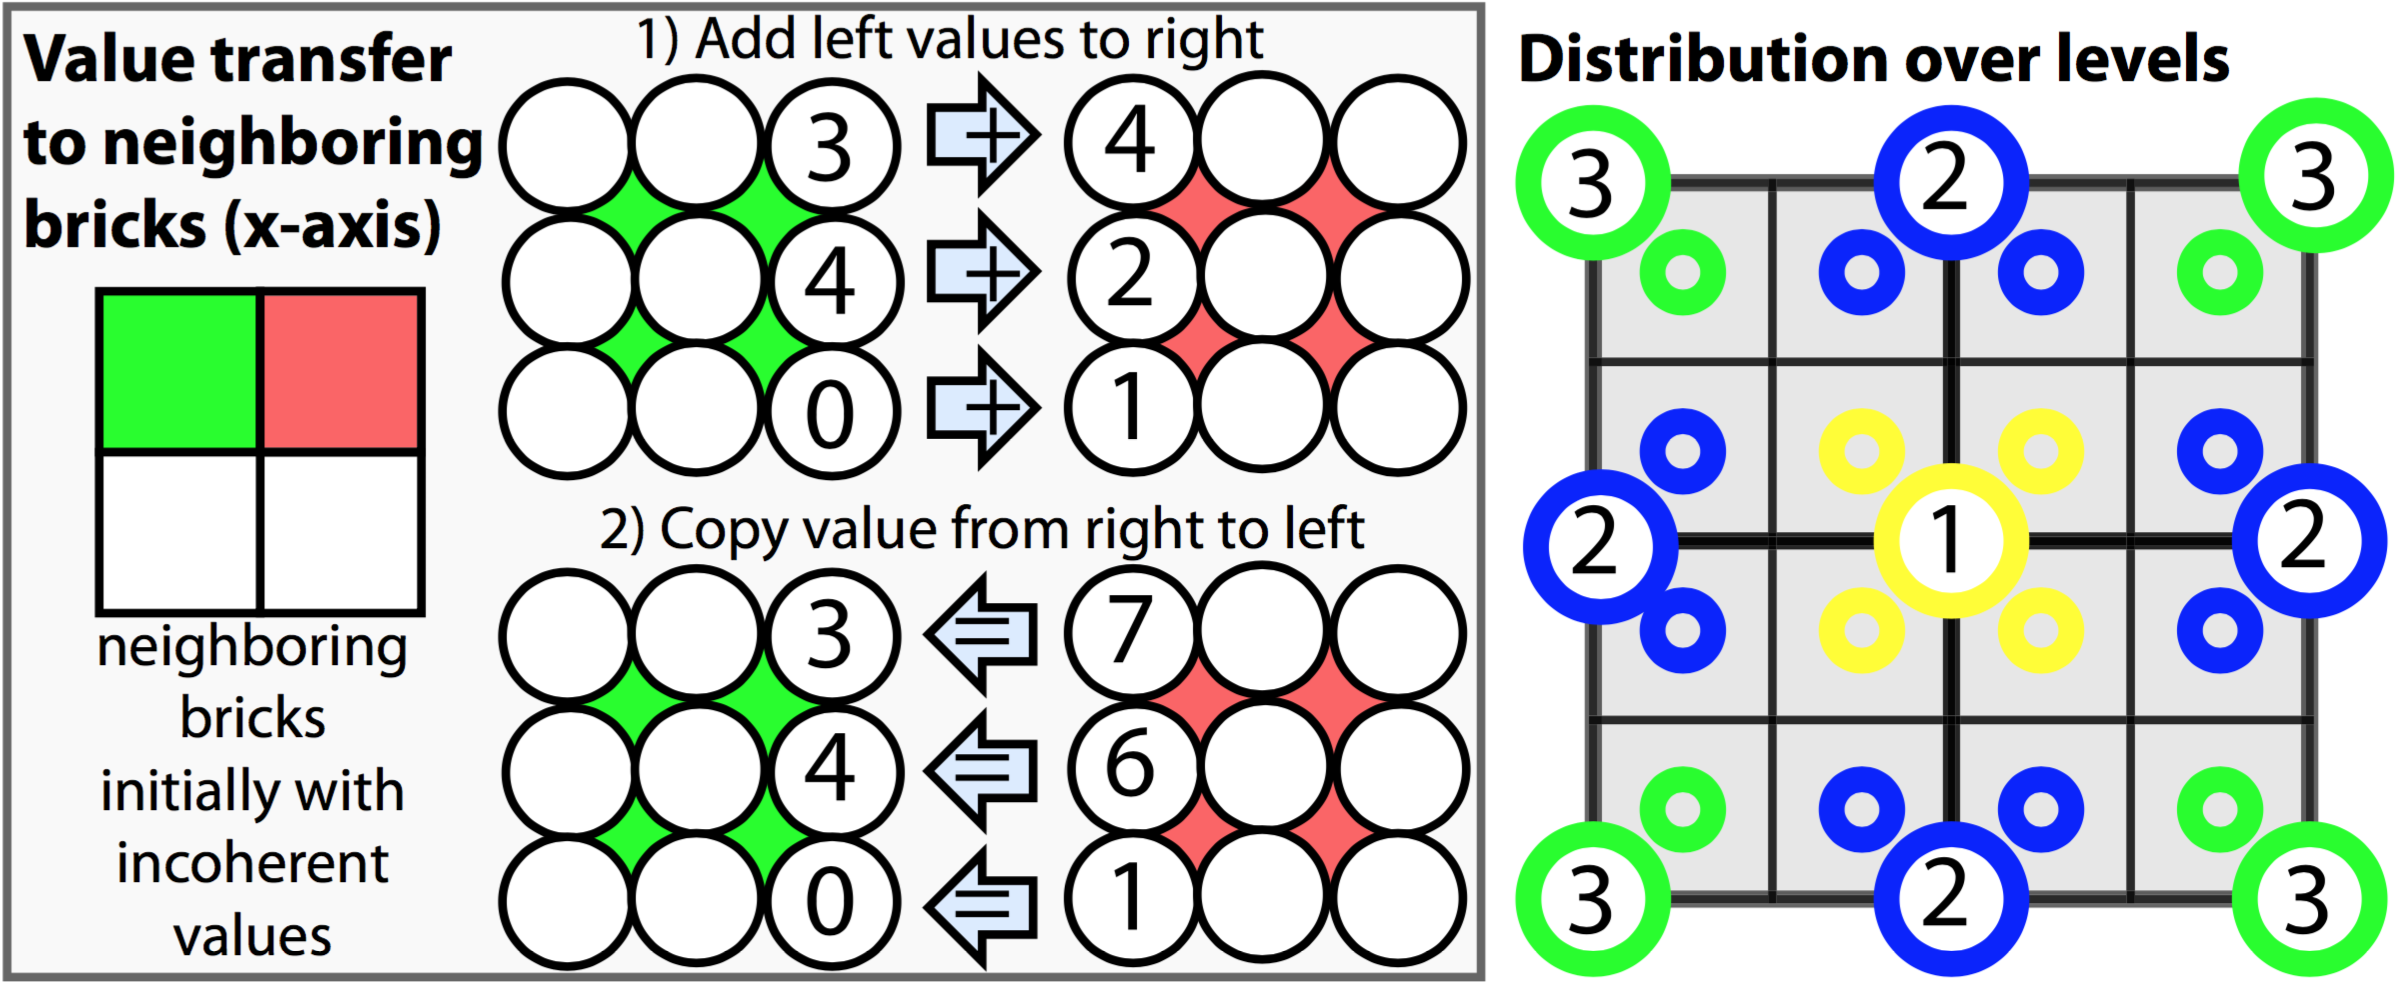
\includegraphics[width=0.9\textwidth]{graphics/vct/vct-14-4}
	\end{center}
	\caption{Left: After photon splatting, an addition and copy along each axis is used to correct inconsistencies on for du- plicated voxels at bricks boundaries. Right: To filter values from a lower to a higher level, three passes are applied (numbers). The threads sum up lower-level voxels (all around the indicated octants);}
\end{figure} 

We will perform six passes, two for each axis $(x,y,z)$. In the first $x$-axis pass, see the left of figure \ref{f:vct-value-transfer}, each thread will add voxel value data from the current node to the corresponding voxels of the brick to its \textit{right}. In practice, this means that three values per thread are added. The next pass for the $x$-axis will transfer data from the right (where we now have the sum) to the left by copying the values. After this step, values along the $x$-axis are coherent and correctly distributed. Repeating the same process for the y and $z$-axis ensures that all voxels have been correctly updated. The approach is very efficient because the neighbor pointers allow us to quickly access neighboring nodes and thread collisions are avoided. In fact, not even atomic operations are needed.




\subsubsection{Distribution Over Levels}
At this point we have coherent information on the lowest level of the octree and the next step is to filter the values and store the result in the higher levels (MIP-map). A simple solution would be to launch one thread on each voxel of the higher level and fetch data from the lower level. Nonetheless, this has an important disadvantage: for shared voxels, the same computations are performed may (up to eight) times. Also, the computation cost of the threads differs depending on the processed voxel leading to an unbalanced scheduling.

Our solution is to perform three separate passes in which all threads have roughly the same cost, see the right of figure \ref{f:vct-value-transfer}. The idea is to only partially compute the filtered results and use the previously-presented transfer between bricks to complete the result. The first pass computes the center voxel using the involved 27 voxels on the lower level (indicated by the yellow octants in figure \ref{f:vct-value-transfer}). The second pass computes \textit{half} of the filtered response for the voxels situated in the center of the node's faces (blue). Because only half the value is computed, only 18 voxel values are involved. Finally, the third pass launches threads for the corner voxels (green) that compute a partial filtering of voxels from a single octant. After these passes, the higher-level voxels are in a similar situation as were the leafs after the initial photon splatting: octree vertices might only contain a part of the result, but summing values across bricks, gives the desired result. Consequently, it is enough to apply the previously-presented transfer step to finalize the filtering.

